%%=============================================================================
%% LaTeX sjabloon voor bachelorproef, HoGent Bedrijf en Organisatie
%% Opleiding Toegepaste Informatica
%%=============================================================================

\documentclass[fleqn,a4paper,12pt]{book}

%%=============================================================================
%% LaTeX sjabloon voor de bachelorproef, HoGent Bedrijf en Organisatie
%% Opleiding toegepaste informatica
%%
%% Structuur en algemene vormgeving. Meestal hoef je hier niets te wijzigen.
%%
%% Vormgeving gebaseerd op "The Legrand Orange Book", version 2.0 (9/2/15)
%% door Mathias Legrand (legrand.mathias@gmail.com) met aanpassingen door
%% Vel (vel@latextemplates.com). Het oorspronkelijke template is te vinden op
%% http://www.LaTeXTemplates.com
%%
%% Aanpassingen voor HoGent toegepaste informatica: 
%%   Bert Van Vreckem <bert.vanvreckem@hogent.be>
%% Licentie: 
%%   CC BY-NC-SA 3.0 (http://creativecommons.org/licenses/by-nc-sa/3.0/)
%%=============================================================================

%%-----------------------------------------------------------------------------
%% Packages
%%-----------------------------------------------------------------------------

\usepackage[top=3cm,bottom=3cm,left=3cm,right=3cm,headsep=10pt,a4paper]{geometry} % Page margins
\usepackage[utf8]{inputenc}  % Accenten gebruiken in tekst (vb. é ipv \'e)
\usepackage{amsfonts}        % AMS math packages: extra wiskundige
\usepackage{amsmath}         %   symbolen (o.a. getallen-
\usepackage{amssymb}         %   verzamelingen N, R, Z, Q, etc.)
\usepackage[english,dutch]{babel}    % Taalinstellingen: woordsplitsingen,
                             %  commando's voor speciale karakters
                             %  ("dutch" voor NL)
\usepackage{iflang}
\usepackage{eurosym}         % Euro-symbool €
\usepackage{geometry}
\usepackage{graphicx}        % Invoegen van tekeningen
\graphicspath{{img/}}       % Specifies the directory where pictures are stored
\usepackage{tikz}            % Required for drawing custom shapes
\usepackage[pdftex,bookmarks=true]{hyperref}
                             % PDF krijgt klikbare links & verwijzingen,
                             %  inhoudstafel
\usepackage{enumitem}        % Customize lists
\setlist{nolistsep}         % Reduce spacing between list items
\usepackage{listings}        % Broncode mooi opmaken
\usepackage{multirow}        % Tekst over verschillende cellen in tabellen
\usepackage{rotating}        % Tabellen en figuren roteren

\usepackage{booktabs}        % Required for nicer horizontal rules in tables

\usepackage{xcolor}          % Required for specifying colors by name
\definecolor{maincolor}{RGB}{0,147,208} % Define the main color used for 
                             % highlighting throughout the book
                             % 0, 147, 208 = officiële kleur HoGent FBO

% Paragraph style: no indent, add space between paragraphs
\setlength{\parindent}{0em}
\setlength{\parskip}{1em}

\usepackage{etoolbox}
\usepackage{titling} % Macros for title, author, etc
\usepackage{lipsum}          % Voor vultekst (lorem ipsum)

% Woordenlijst
\usepackage[toc]{glossaries}

% Tree
\usepackage{qtree}

\lstdefinestyle{command_style}{
  basicstyle=\ttfamily\footnotesize,
  breaklines=true,
  showstringspaces=false
}

% SVG
\usepackage{svg}

%----------------------------------------------------------------------------------------
%	FONTS
%----------------------------------------------------------------------------------------

\usepackage{avant} % Use the Avantgarde font for headings
%\usepackage{times} % Use the Times font for headings
\usepackage{mathptmx} % Use the Adobe Times Roman as the default text font together with math symbols from the Sym­bol, Chancery and Com­puter Modern fonts

\usepackage{microtype} % Slightly tweak font spacing for aesthetics
\usepackage[utf8]{inputenc} % Required for including letters with accents
\usepackage[T1]{fontenc} % Use 8-bit encoding that has 256 glyphs

%------------------------------------------------------------------------------
%	TITLE PAGE
%------------------------------------------------------------------------------

\newcommand{\inserttitlepage}{%
\begin{titlepage}
  \newgeometry{top=2cm,bottom=1.5cm,left=1.5cm,right=1.5cm}
  \begin{center}

    \begingroup
    \rmfamily
    \includegraphics[width=2.5cm]{img/HG-beeldmerk-woordmerk}\\[.5cm]
    Faculteit Bedrijf en Organisatie\\[3cm]
    \titel
    \vfill
    \student\\[3.5cm]
    Scriptie voorgedragen tot het bekomen van de graad van\\professionele bachelor in de toegepaste informatica\\[2cm]
    Promotor:\\
    \promotor\\
    \ifdefempty{\copromotor}{\vspace{2.5cm}}{Co-promotor:\\\copromotor\\[2.5cm]}
    Instelling: \instelling\\[.5cm]
    Academiejaar: \academiejaar\\[.5cm]
    \ifcase \examenperiode \or Eerste \or Tweede \else Derde \fi examenperiode
    \endgroup

  \end{center}
  \restoregeometry
\end{titlepage}
  \emptypage
\begin{titlepage}
  \newgeometry{top=5.35cm,bottom=1.5cm,left=1.5cm,right=1.5cm}
  \begin{center}

    \begingroup
    \rmfamily
    \IfLanguageName{dutch}{Faculteit Bedrijf en Organisatie}{Faculty of Business and Information Management}\\[3cm]
    \titel
    \vfill
    \student\\[3.5cm]
    \IfLanguageName{dutch}{Scriptie voorgedragen tot het bekomen van de graad van\\professionele bachelor in de toegepaste informatica}{Thesis submitted in partial fulfillment of the requirements for the degree of\\professional bachelor of applied computer science}\\[2cm]
    Promotor:\\
    \promotor\\
    \ifdefempty{\copromotor}{\vspace{2.5cm}}{Co-promotor:\\\copromotor\\[2.5cm]}
    \IfLanguageName{dutch}{Instelling}{Institution}: \instelling\\[.5cm]
    \IfLanguageName{dutch}{Academiejaar}{Academic year}: \academiejaar\\[.5cm]
    \IfLanguageName{dutch}{%
    \ifcase \examenperiode \or Eerste \or Tweede \else Derde \fi examenperiode}{%
    \ifcase \examenperiode \or First \or Second \else Third \fi examination period}
    \endgroup

  \end{center}
  \restoregeometry
\end{titlepage}
}

%----------------------------------------------------------------------------------------
%	BIBLIOGRAPHY AND INDEX
%----------------------------------------------------------------------------------------

\usepackage[style=apa,backend=biber]{biblatex}
\usepackage{csquotes}
\DeclareLanguageMapping{dutch}{dutch-apa}
\addbibresource{bachproef-tin.bib} % BibTeX bibliography file
\defbibheading{bibempty}{}

\usepackage{calc} % For simpler calculation - used for spacing the index letter headings correctly
\usepackage{makeidx} % Required to make an index
\makeindex % Tells LaTeX to create the files required for indexing

%----------------------------------------------------------------------------------------
%	MAIN TABLE OF CONTENTS
%----------------------------------------------------------------------------------------

\usepackage{titletoc} % Required for manipulating the table of contents

\contentsmargin{0cm} % Removes the default margin

% Part text styling
\titlecontents{part}[0cm]
{\addvspace{20pt}\centering\large\bfseries}
{}
{}
{}

% Chapter text styling
\titlecontents{chapter}[1.25cm] % Indentation
{\addvspace{12pt}\large\sffamily\bfseries} % Spacing and font options for chapters
{\color{maincolor!60}\contentslabel[\Large\thecontentslabel]{1.25cm}\color{maincolor}} % Chapter number
{\color{maincolor}}
{\color{maincolor!60}\normalsize\;\titlerule*[.5pc]{.}\;\thecontentspage} % Page number

% Section text styling
\titlecontents{section}[1.25cm] % Indentation
{\addvspace{3pt}\sffamily\bfseries} % Spacing and font options for sections
{\contentslabel[\thecontentslabel]{1.25cm}} % Section number
{}
{\hfill\color{black}\thecontentspage} % Page number
[]

% Subsection text styling
\titlecontents{subsection}[1.25cm] % Indentation
{\addvspace{1pt}\sffamily\small} % Spacing and font options for subsections
{\contentslabel[\thecontentslabel]{1.25cm}} % Subsection number
{}
{\ \titlerule*[.5pc]{.}\;\thecontentspage} % Page number
[]

% List of figures
\titlecontents{figure}[0em]
{\addvspace{-5pt}\sffamily}
{\thecontentslabel\hspace*{1em}}
{}
{\ \titlerule*[.5pc]{.}\;\thecontentspage}
[]

% List of tables
\titlecontents{table}[0em]
{\addvspace{-5pt}\sffamily}
{\thecontentslabel\hspace*{1em}}
{}
{\ \titlerule*[.5pc]{.}\;\thecontentspage}
[]

%----------------------------------------------------------------------------------------
%	MINI TABLE OF CONTENTS IN PART HEADS
%----------------------------------------------------------------------------------------

% Chapter text styling
\titlecontents{lchapter}[0em] % Indenting
{\addvspace{15pt}\large\sffamily\bfseries} % Spacing and font options for chapters
{\color{maincolor}\contentslabel[\Large\thecontentslabel]{1.25cm}\color{maincolor}} % Chapter number
{}
{\color{maincolor}\normalsize\sffamily\bfseries\;\titlerule*[.5pc]{.}\;\thecontentspage} % Page number

% Section text styling
\titlecontents{lsection}[0em] % Indenting
{\sffamily\small} % Spacing and font options for sections
{\contentslabel[\thecontentslabel]{1.25cm}} % Section number
{}
{}

% Subsection text styling
\titlecontents{lsubsection}[.5em] % Indentation
{\normalfont\footnotesize\sffamily} % Font settings
{}
{}
{}

%----------------------------------------------------------------------------------------
%	PAGE HEADERS
%----------------------------------------------------------------------------------------

\usepackage{fancyhdr} % Required for header and footer configuration

\pagestyle{fancy}
\renewcommand{\chaptermark}[1]{\markboth{\sffamily\normalsize\bfseries\chaptername\ \thechapter.\ #1}{}} % Chapter text font settings
\renewcommand{\sectionmark}[1]{\markright{\sffamily\normalsize\thesection\hspace{5pt}#1}{}} % Section text font settings
\fancyhf{} \fancyhead[LE,RO]{\sffamily\normalsize\thepage} % Font setting for the page number in the header
\fancyhead[LO]{\rightmark} % Print the nearest section name on the left side of odd pages
\fancyhead[RE]{\leftmark} % Print the current chapter name on the right side of even pages
\renewcommand{\headrulewidth}{0.5pt} % Width of the rule under the header
\addtolength{\headheight}{2.5pt} % Increase the spacing around the header slightly
\renewcommand{\footrulewidth}{0pt} % Removes the rule in the footer
\fancypagestyle{plain}{\fancyhead{}\renewcommand{\headrulewidth}{0pt}} % Style for when a plain pagestyle is specified

% Removes the header from odd empty pages at the end of chapters
\makeatletter
\renewcommand{\cleardoublepage}{
\clearpage\ifodd\c@page\else
\hbox{}
\vspace*{\fill}
\thispagestyle{empty}
\newpage
\fi}

%----------------------------------------------------------------------------------------
%	THEOREM STYLES
%----------------------------------------------------------------------------------------

\usepackage{amsmath,amsfonts,amssymb,amsthm} % For math equations, theorems, symbols, etc

\newcommand{\intoo}[2]{\mathopen{]}#1\,;#2\mathclose{[}}
\newcommand{\ud}{\mathop{\mathrm{{}d}}\mathopen{}}
\newcommand{\intff}[2]{\mathopen{[}#1\,;#2\mathclose{]}}
\newtheorem{notation}{Notation}[chapter]

% Boxed/framed environments
\newtheoremstyle{maincolornumbox}% % Theorem style name
{0pt}% Space above
{0pt}% Space below
{\normalfont}% % Body font
{}% Indent amount
{\small\bf\sffamily\color{maincolor}}% % Theorem head font
{\;}% Punctuation after theorem head
{0.25em}% Space after theorem head
{\small\sffamily\color{maincolor}\thmname{#1}\nobreakspace\thmnumber{\@ifnotempty{#1}{}\@upn{#2}}% Theorem text (e.g. Theorem 2.1)
\thmnote{\nobreakspace\the\thm@notefont\sffamily\bfseries\color{black}---\nobreakspace#3.}} % Optional theorem note
\renewcommand{\qedsymbol}{$\blacksquare$}% Optional qed square

\newtheoremstyle{blacknumex}% Theorem style name
{5pt}% Space above
{5pt}% Space below
{\normalfont}% Body font
{} % Indent amount
{\small\bf\sffamily}% Theorem head font
{\;}% Punctuation after theorem head
{0.25em}% Space after theorem head
{\small\sffamily{\tiny\ensuremath{\blacksquare}}\nobreakspace\thmname{#1}\nobreakspace\thmnumber{\@ifnotempty{#1}{}\@upn{#2}}% Theorem text (e.g. Theorem 2.1)
\thmnote{\nobreakspace\the\thm@notefont\sffamily\bfseries---\nobreakspace#3.}}% Optional theorem note

\newtheoremstyle{blacknumbox} % Theorem style name
{0pt}% Space above
{0pt}% Space below
{\normalfont}% Body font
{}% Indent amount
{\small\bf\sffamily}% Theorem head font
{\;}% Punctuation after theorem head
{0.25em}% Space after theorem head
{\small\sffamily\thmname{#1}\nobreakspace\thmnumber{\@ifnotempty{#1}{}\@upn{#2}}% Theorem text (e.g. Theorem 2.1)
\thmnote{\nobreakspace\the\thm@notefont\sffamily\bfseries---\nobreakspace#3.}}% Optional theorem note

% Non-boxed/non-framed environments
\newtheoremstyle{maincolornum}% % Theorem style name
{5pt}% Space above
{5pt}% Space below
{\normalfont}% % Body font
{}% Indent amount
{\small\bf\sffamily\color{maincolor}}% % Theorem head font
{\;}% Punctuation after theorem head
{0.25em}% Space after theorem head
{\small\sffamily\color{maincolor}\thmname{#1}\nobreakspace\thmnumber{\@ifnotempty{#1}{}\@upn{#2}}% Theorem text (e.g. Theorem 2.1)
\thmnote{\nobreakspace\the\thm@notefont\sffamily\bfseries\color{black}---\nobreakspace#3.}} % Optional theorem note
\renewcommand{\qedsymbol}{$\blacksquare$}% Optional qed square
\makeatother

% Defines the theorem text style for each type of theorem to one of the three styles above
\newcounter{dummy}
\numberwithin{dummy}{section}
\theoremstyle{maincolornumbox}
\newtheorem{theoremeT}[dummy]{Theorem}
\newtheorem{problem}{Problem}[chapter]
\newtheorem{exerciseT}{Exercise}[chapter]
\theoremstyle{blacknumex}
\newtheorem{exampleT}{Example}[chapter]
\theoremstyle{blacknumbox}
\newtheorem{vocabulary}{Vocabulary}[chapter]
\newtheorem{definitionT}{Definition}[section]
\newtheorem{corollaryT}[dummy]{Corollary}
\theoremstyle{maincolornum}
\newtheorem{proposition}[dummy]{Proposition}

%----------------------------------------------------------------------------------------
%	DEFINITION OF COLORED BOXES
%----------------------------------------------------------------------------------------

\RequirePackage[framemethod=default]{mdframed} % Required for creating the theorem, definition, exercise and corollary boxes

% Theorem box
\newmdenv[skipabove=7pt,
skipbelow=7pt,
backgroundcolor=black!5,
linecolor=maincolor,
innerleftmargin=5pt,
innerrightmargin=5pt,
innertopmargin=5pt,
leftmargin=0cm,
rightmargin=0cm,
innerbottommargin=5pt]{tBox}

% Exercise box
\newmdenv[skipabove=7pt,
skipbelow=7pt,
rightline=false,
leftline=true,
topline=false,
bottomline=false,
backgroundcolor=maincolor!10,
linecolor=maincolor,
innerleftmargin=5pt,
innerrightmargin=5pt,
innertopmargin=5pt,
innerbottommargin=5pt,
leftmargin=0cm,
rightmargin=0cm,
linewidth=4pt]{eBox}

% Definition box
\newmdenv[skipabove=7pt,
skipbelow=7pt,
rightline=false,
leftline=true,
topline=false,
bottomline=false,
linecolor=maincolor,
innerleftmargin=5pt,
innerrightmargin=5pt,
innertopmargin=0pt,
leftmargin=0cm,
rightmargin=0cm,
linewidth=4pt,
innerbottommargin=0pt]{dBox}

% Corollary box
\newmdenv[skipabove=7pt,
skipbelow=7pt,
rightline=false,
leftline=true,
topline=false,
bottomline=false,
linecolor=gray,
backgroundcolor=black!5,
innerleftmargin=5pt,
innerrightmargin=5pt,
innertopmargin=5pt,
leftmargin=0cm,
rightmargin=0cm,
linewidth=4pt,
innerbottommargin=5pt]{cBox}

% Creates an environment for each type of theorem and assigns it a theorem text style from the "Theorem Styles" section above and a colored box from above
\newenvironment{theorem}{\begin{tBox}\begin{theoremeT}}{\end{theoremeT}\end{tBox}}
\newenvironment{exercise}{\begin{eBox}\begin{exerciseT}}{\hfill{\color{maincolor}\tiny\ensuremath{\blacksquare}}\end{exerciseT}\end{eBox}}
\newenvironment{definition}{\begin{dBox}\begin{definitionT}}{\end{definitionT}\end{dBox}}
\newenvironment{example}{\begin{exampleT}}{\hfill{\tiny\ensuremath{\blacksquare}}\end{exampleT}}
\newenvironment{corollary}{\begin{cBox}\begin{corollaryT}}{\end{corollaryT}\end{cBox}}

%----------------------------------------------------------------------------------------
%	REMARK ENVIRONMENT
%----------------------------------------------------------------------------------------

\newenvironment{remark}{\par\vspace{10pt}\small % Vertical white space above the remark and smaller font size
\begin{list}{}{
\leftmargin=35pt % Indentation on the left
\rightmargin=25pt}\item\ignorespaces % Indentation on the right
\makebox[-2.5pt]{\begin{tikzpicture}[overlay]
\node[draw=maincolor!60,line width=1pt,circle,fill=maincolor!25,font=\sffamily\bfseries,inner sep=2pt,outer sep=0pt] at (-15pt,0pt){\textcolor{maincolor}{R}};\end{tikzpicture}} % Orange R in a circle
\advance\baselineskip -1pt}{\end{list}\vskip5pt} % Tighter line spacing and white space after remark

%----------------------------------------------------------------------------------------
%	SECTION NUMBERING IN THE MARGIN
%----------------------------------------------------------------------------------------

\makeatletter
\renewcommand{\@seccntformat}[1]{\llap{\textcolor{maincolor}{\csname the#1\endcsname}\hspace{1em}}}
\renewcommand{\section}{\@startsection{section}{1}{\z@}
{-4ex \@plus -1ex \@minus -.4ex}
{1ex \@plus.2ex }
{\normalfont\large\sffamily\bfseries}}
\renewcommand{\subsection}{\@startsection {subsection}{2}{\z@}
{-3ex \@plus -0.1ex \@minus -.4ex}
{0.5ex \@plus.2ex }
{\normalfont\sffamily\bfseries}}
\renewcommand{\subsubsection}{\@startsection {subsubsection}{3}{\z@}
{-2ex \@plus -0.1ex \@minus -.2ex}
{.2ex \@plus.2ex }
{\normalfont\small\sffamily\bfseries}}
\renewcommand\paragraph{\@startsection{paragraph}{4}{\z@}
{-2ex \@plus-.2ex \@minus .2ex}
{.1ex}
{\normalfont\small\sffamily\bfseries}}

%----------------------------------------------------------------------------------------
%	PART HEADINGS
%----------------------------------------------------------------------------------------

% numbered part in the table of contents
\newcommand{\@mypartnumtocformat}[2]{%
\setlength\fboxsep{0pt}%
\noindent\colorbox{maincolor!20}{\strut\parbox[c][.7cm]{\ecart}{\color{maincolor!70}\Large\sffamily\bfseries\centering#1}}\hskip\esp\colorbox{maincolor!40}{\strut\parbox[c][.7cm]{\linewidth-\ecart-\esp}{\Large\sffamily\centering#2}}}%
%%%%%%%%%%%%%%%%%%%%%%%%%%%%%%%%%%
% unnumbered part in the table of contents
\newcommand{\@myparttocformat}[1]{%
\setlength\fboxsep{0pt}%
\noindent\colorbox{maincolor!40}{\strut\parbox[c][.7cm]{\linewidth}{\Large\sffamily\centering#1}}}%
%%%%%%%%%%%%%%%%%%%%%%%%%%%%%%%%%%
\newlength\esp
\setlength\esp{4pt}
\newlength\ecart
\setlength\ecart{1.2cm-\esp}
\newcommand{\thepartimage}{}%
\newcommand{\partimage}[1]{\renewcommand{\thepartimage}{#1}}%
\def\@part[#1]#2{%
\ifnum \c@secnumdepth >-2\relax%
\refstepcounter{part}%
\addcontentsline{toc}{part}{\texorpdfstring{\protect\@mypartnumtocformat{\thepart}{#1}}{\partname~\thepart\ ---\ #1}}
\else%
\addcontentsline{toc}{part}{\texorpdfstring{\protect\@myparttocformat{#1}}{#1}}%
\fi%
\startcontents%
\markboth{}{}%
{\thispagestyle{empty}%
\begin{tikzpicture}[remember picture,overlay]%
\node at (current page.north west){\begin{tikzpicture}[remember picture,overlay]%
\fill[maincolor!20](0cm,0cm) rectangle (\paperwidth,-\paperheight);
\node[anchor=north] at (4cm,-3.25cm){\color{maincolor!40}\fontsize{220}{100}\sffamily\bfseries\@Roman\c@part};
\node[anchor=south east] at (\paperwidth-1cm,-\paperheight+1cm){\parbox[t][][t]{8.5cm}{
\printcontents{l}{0}{\setcounter{tocdepth}{1}}%
}};
\node[anchor=north east] at (\paperwidth-1.5cm,-3.25cm){\parbox[t][][t]{15cm}{\strut\raggedleft\color{white}\fontsize{30}{30}\sffamily\bfseries#2}};
\end{tikzpicture}};
\end{tikzpicture}}%
\@endpart}
\def\@spart#1{%
\startcontents%
\phantomsection
{\thispagestyle{empty}%
\begin{tikzpicture}[remember picture,overlay]%
\node at (current page.north west){\begin{tikzpicture}[remember picture,overlay]%
\fill[maincolor!20](0cm,0cm) rectangle (\paperwidth,-\paperheight);
\node[anchor=north east] at (\paperwidth-1.5cm,-3.25cm){\parbox[t][][t]{15cm}{\strut\raggedleft\color{white}\fontsize{30}{30}\sffamily\bfseries#1}};
\end{tikzpicture}};
\end{tikzpicture}}
\addcontentsline{toc}{part}{\texorpdfstring{%
\setlength\fboxsep{0pt}%
\noindent\protect\colorbox{maincolor!40}{\strut\protect\parbox[c][.7cm]{\linewidth}{\Large\sffamily\protect\centering #1\quad\mbox{}}}}{#1}}%
\@endpart}
\def\@endpart{\vfil\newpage
\if@twoside
\if@openright
\null
\thispagestyle{empty}%
\newpage
\fi
\fi
\if@tempswa
\twocolumn
\fi}

%----------------------------------------------------------------------------------------
%	CHAPTER HEADINGS
%----------------------------------------------------------------------------------------

% A switch to conditionally include a picture, implemented by  Christian Hupfer
\newif\ifusechapterimage
\usechapterimagetrue
\newcommand{\thechapterimage}{}%
\newcommand{\chapterimage}[1]{\ifusechapterimage\renewcommand{\thechapterimage}{#1}\fi}%
\def\@makechapterhead#1{%
{\parindent \z@ \raggedright \normalfont
\ifnum \c@secnumdepth >\m@ne
\if@mainmatter
\begin{tikzpicture}[remember picture,overlay]
\node at (current page.north west)
{\begin{tikzpicture}[remember picture,overlay]
\node[anchor=north west,inner sep=0pt] at (0,0) {\ifusechapterimage\includegraphics[width=\paperwidth]{\thechapterimage}\fi};
\draw[anchor=west] (\Gm@lmargin,-9cm) node [line width=2pt,rounded corners=15pt,draw=maincolor,fill=white,fill opacity=0.5,inner sep=15pt]{\strut\makebox[22cm]{}};
\draw[anchor=west] (\Gm@lmargin+.3cm,-9cm) node {\huge\sffamily\bfseries\color{black}\thechapter. #1\strut};
\end{tikzpicture}};
\end{tikzpicture}
\else
\begin{tikzpicture}[remember picture,overlay]
\node at (current page.north west)
{\begin{tikzpicture}[remember picture,overlay]
\node[anchor=north west,inner sep=0pt] at (0,0) {\ifusechapterimage\includegraphics[width=\paperwidth]{\thechapterimage}\fi};
\draw[anchor=west] (\Gm@lmargin,-9cm) node [line width=2pt,rounded corners=15pt,draw=maincolor,fill=white,fill opacity=0.5,inner sep=15pt]{\strut\makebox[22cm]{}};
\draw[anchor=west] (\Gm@lmargin+.3cm,-9cm) node {\huge\sffamily\bfseries\color{black}#1\strut};
\end{tikzpicture}};
\end{tikzpicture}
\fi\fi\par\vspace*{270\p@}}}

%-------------------------------------------

\def\@makeschapterhead#1{%
\begin{tikzpicture}[remember picture,overlay]
\node at (current page.north west)
{\begin{tikzpicture}[remember picture,overlay]
\node[anchor=north west,inner sep=0pt] at (0,0) {\ifusechapterimage\includegraphics[width=\paperwidth]{\thechapterimage}\fi};
\draw[anchor=west] (\Gm@lmargin,-9cm) node [line width=2pt,rounded corners=15pt,draw=maincolor,fill=white,fill opacity=0.5,inner sep=15pt]{\strut\makebox[22cm]{}};
\draw[anchor=west] (\Gm@lmargin+.3cm,-9cm) node {\huge\sffamily\bfseries\color{black}#1\strut};
\end{tikzpicture}};
\end{tikzpicture}
\par\vspace*{270\p@}}
\makeatother

%----------------------------------------------------------------------------------------
%	HYPERLINKS IN THE DOCUMENTS
%----------------------------------------------------------------------------------------

\usepackage{hyperref}
\hypersetup{hidelinks,backref=true,pagebackref=true,hyperindex=true,colorlinks=false,breaklinks=true,urlcolor= maincolor,bookmarks=true,bookmarksopen=false,pdftitle={Title},pdfauthor={Author}}
\usepackage{bookmark}
\bookmarksetup{
open,
numbered,
addtohook={%
\ifnum\bookmarkget{level}=0 % chapter
\bookmarksetup{bold}%
\fi
\ifnum\bookmarkget{level}=-1 % part
\bookmarksetup{color=maincolor,bold}%
\fi
}
}

%----------------------------------------------------------------------------------------
%	Java source code
%----------------------------------------------------------------------------------------

% Commando voor invoegen Java-broncodebestanden (dank aan Niels Corneille)
% Gebruik:
%   \codefragment{source/MijnKlasse.java}{Uitleg bij de code}
%
% Je kan dit aanpassen aan de taal die je zelf het meeste gebruikt in je
% bachelorproef.
\newcommand{\codefragment}[2]{ \lstset{%
  language=bash,
  breaklines=true,
  float=th,
  caption={#2},
  basicstyle=\scriptsize,
  frame=single,
  extendedchars=\true
}
\lstinputlisting{#1}}

% Leeg blad
\newcommand{\emptypage}{%
\newpage
\thispagestyle{empty}
\mbox{}
\newpage
}


%%---------- Documenteigenschappen --------------------------------------------
%% TODO: Vul dit aan met je eigen info:

% Je eigen naam
\newcommand{\student}{Jonas De Moor}

% De naam van je promotor (lector van de opleiding)
\newcommand{\promotor}{Antonia Pierreux}

% De naam van je co-promotor. Als je promotor ook je opdrachtgever is en je
% dus ook inhoudelijk begeleidt (en enkel dan!), mag je dit leeg laten.
\newcommand{\copromotor}{Karine Van Driessche}

% Indien je bachelorproef in opdracht van/in samenwerking met een bedrijf of
% externe organisatie geschreven is, geef je hier de naam. Zoniet laat je dit
% zoals het is.
\newcommand{\instelling}{---}

% De titel van het rapport/bachelorproef
\newcommand{\titel}{ZFS met RAID-Z als alternatief voor klassieke RAID-oplossingen}

% Datum van indienen (gebruik telkens de deadline, ook al geef je eerder af)
\newcommand{\datum}{2 juni 2017}

% Academiejaar
\newcommand{\academiejaar}{2016-2017}

% Examenperiode
%  - 1e semester = 1e examenperiode => 1
%  - 2e semester = 2e examenperiode => 2
%  - tweede zit  = 3e examenperiode => 3
\newcommand{\examenperiode}{2}


% Woordenlijst

% Andere naam voor woordenlijst
%\renewcommand{\glossaryname}{Gebruikte termen}

\newglossaryentry{performantie}
{
  name={performantie},
  description={Performantie (Engels: performance) is een vrij uitgebreid begrip in de informatica. In het algemeen bedoelt men met performantie meestal hoe goed een computersysteem vooropgestelde taken kan uitvoeren in een bepaalde situatie. Bij het meten van performantie van een systeem kan men één of meerdere aspecten beschouwen: bij schijven kan bijvoorbeeld het aantal I/O's (Invoer- en uitvoerbewerkingen) worden genomen als maatstaf; bij CPU's kan een maatstaf bijvoorbeeld het aantal instructies per seconde zijn dat deze kan verwerken}
}

\newglossaryentry{betrouwbaarheid}
{
  name={betrouwbaarheid},
  description={Betrouwbaarheid (Engels: reliability) heeft betrekking op de betrouwbaarheid van een computersysteem, i.e. of deze al dan niet zijn taken op een juiste manier uitvoert. Men kan bijvoorbeeld stellen dat er zich bij een computersysteem een X aantal fouten mogen voordoen; als deze grens overschreden wordt, dan wordt het systeem als onbetrouwbaar verklaard. Daarnaast heeft betrouwbaarheid ook te maken met de handelswijze van een systeem indien er zich een fout voordoet: men kan zich bijvoorbeeld afvragen hoe er zou moeten gereageerd worden op een kritieke fout en hiervoor test cases opstellen om de betrouwbaarheid van het systeem te testen}
}

\newglossaryentry{capaciteit}
{
  name={capaciteit},
  description={In de context van schijven of RAID-systemen kan capaciteit (Engels: capacity) een aantal betekenissen hebben. In deze scriptie wordt er vooral gesproken over de bruikbare capaciteit van een schijf of RAID-array: dit is de hoeveelheid schijfruimte die kan gebruikt worden door gebruikers om data op te slaan. Daarnaast kan men ook spreken over de totale capaciteit: dit is de som van de gebruikte schijfruimte en de vrije schijfruimte. In theorie is de totale capaciteit van een schijf gelijk aan de werkelijke grootte van een schijf}
}

\newglossaryentry{atomair}
{
  name={atomair},
  description={In de informatica betekent atomiciteit (Engels: atomicity) hetzelfde als ondeelbaarheid; vaak wordt dit begrip ook omschreven als een "alles-of-niets" aanpak. In de context van bijvoorbeeld databanksystemen heeft atomiciteit betrekking op o.a. transacties: ofwel verloopt een transactie succesvol, ofwel mislukt deze (door bv. een onderbreking) en moet de databank kunnen teruggebracht worden naar een consistente toestand. Meestal betekent dit dan dat er een rollback moet worden uitgevoerd} 
}

\newglossaryentry{bottleneck}
{
  name={bottleneck},
  description={Een bottleneck (letterlijk vertaald 'flessenhals') is een begrip dat gebruikt wordt om een onderdeel van een systeem aan te duiden dat andere onderdelen hindert en/of vertraagt. Dit begrip wordt ook vaak gebruikt in de zelfbouw PC community om een computeronderdeel aan te duiden dat de computer ervan verhindert om optimaal te kunnen presteren: zo kan het samen gebruiken van een oude CPU en een nieuwe GPU ertoe leiden dat de computer niet optimaal presteert bij bijvoorbeeld games. In dit geval wordt de CPU de bottleneck van het systeem genoemd}
}

\newglossaryentry{striping}
{
  name={striping},
  description={Striping heeft betrekking op de manier waarop blokken data verdeeld worden over een reeks van schijven door bijvoorbeeld een RAID-controller (hetzij hardwarematig, hetzij softwarematig). Datablokken die verdeeld zijn over meerdere schijven en samen één geheel vormen worden een stripe genoemd}
}

\newglossaryentry{parity}
{
  name={parity},
  description={Parity is een foutdetectiemechanisme dat gebruikt wordt om in geval van bijvoorbeeld datacorruptie de originele data te reconstrueren. Bij RAID gebruikt men parityblokken: dit zijn blokken metadata die worden berekend door een mathematische functie (meestal een XOR-functie) uit te voeren op de opgeslagen data. Zo kan een RAID-controller de originele data reconstrueren indien er een schijf wordt vervangen in een RAID-array}
}

\newglossaryentry{round-robin}
{
  name={round-robin},
  description={In de informatica is round-robin een scheduling-algoritme dat o.a. gebruikt wordt in besturingssystemen. Bij round-robin krijgt elk proces om de beurt een gelijk stukje processortijd. Hierdoor treedt er bij deze vorm van scheduling geen \textit{starvation} op. Starvation is een fenomeen waarbij een proces te weinig of helemaal geen processortijd krijgt om zijn taken uit te voeren; het proces wordt a.h.w. "uitgehongerd" doordat het geen resources krijgt van het OS}
}

\newglossaryentry{workload}
{
  name={workload},
  description={De workload van een systeem heeft in het algemeen betrekking op de hoeveelheid werk dat een systeem moet verrichten onder bepaalde omstandigheden. In deze scriptie wordt er met 'workload' vooral de toepassingen bedoeld die op het systeem draaien; onder deze workload worden dan een reeks testen uitgevoerd om verschillende aspecten van het testsysteem te analyseren}
}

\newglossaryentry{journal}
{
  name={journal},
  description={Een journal is een soort logboek dat door journaling bestandssystemen (zoals EXT4) wordt bijgehouden. In een journal worden alle transacties die op een bepaald moment aan het lopen zijn gelogd; bij een crash of andere onderbreking kan het bestandssysteem worden hersteld naar een consistente toestand door het journal na te kijken en transacties terug te rollen}
}

\newglossaryentry{fsync}
{
  name={fsync},
  description={Op UNIX en UNIX-achtige systemen is \texttt{sync} of \texttt{fsync} een system call dat gebufferde data dat zich in het RAM-geheugen bevindt flusht naar opslagapparaten. Door deze call uit te voeren wordt data die zich in het werkgeheugen bevindt - en zich dus in een vluchtige toestand bevindt - gepersisteerd en niet-vluchtig gemaakt}
}

\newglossaryentry{checksum}
{
  name={checksum},
  description={Een checksum is een (meestal) klein gegeven dat dient om de dataintegriteit van een ander bestand te garanderen. Indien er tijdens het verzenden van een bestand bijvoorbeeld fouten optreden, dan kan dit met behulp van deze checksum worden gedetecteerd: bij aankomst wordt de checksum herberekend en vergeleken met de originele tekenreeks. Deze tekenreeks wordt berekend met behulp van een cryptografische functie dat het bestand in kwestie als invoer neemt. Zelfs bij een kleine wijziging aan het bestand, zal een herberekening van de checksum leiden tot een andere tekenreeks dan de originele}
}

\newglossaryentry{fsck}
{
  name={fsck},
  description={\texttt{fsck} (acroniem voor 'filesystem consistency check') is een programma op UNIX en UNIX-achtige systemen dat bestandssystemen controleert op consistentie. Dit programma kan manueel worden gedraaid door de systeembeheerder, maar in de meeste gevallen wordt dit programma automatisch opgeroepen bij het opstarten van het systeem. \texttt{fsck} werkt op bestandssysteemniveau en dus heeft elk bestandssysteem een eigen,specifieke implementatie van dit programma}
}

\makenoidxglossaries

%%=============================================================================
%% Inhoud document
%%=============================================================================

\begin{document}

%---------- Taalselectie ------------------------------------------------------
%% Als je je bachelorproef in het Engels schrijft, haal dan onderstaande regel
%% uit commentaar. Let op: de tekst op de voorkaft blijft in het Nederlands, en
%% dat is ook de bedoeling!
%\selectlanguage{english}

%---------- Titelblad ---------------------------------------------------------
\inserttitlepage

%---------- Samenvatting, voorwoord -------------------------------------------
\usechapterimagefalse
%%=============================================================================
%% Samenvatting
%%=============================================================================

%% TODO: De "abstract" of samenvatting is een kernachtige (~ 1 blz. voor een
%% thesis) synthese van het document.
%%
%% Deze aspecten moeten zeker aan bod komen:
%% - Context: waarom is dit werk belangrijk?
%% - Nood: waarom moest dit onderzocht worden?
%% - Taak: wat heb je precies gedaan?
%% - Object: wat staat in dit document geschreven?
%% - Resultaat: wat was het resultaat?
%% - Conclusie: wat is/zijn de belangrijkste conclusie(s)?
%% - Perspectief: blijven er nog vragen open die in de toekomst nog kunnen
%%    onderzocht worden? Wat is een mogelijk vervolg voor jouw onderzoek?
%%
%% LET OP! Een samenvatting is GEEN voorwoord!

%%---------- Nederlandse samenvatting -----------------------------------------
%%
%% TODO: Als je je bachelorproef in het Engels schrijft, moet je eerst een
%% Nederlandse samenvatting invoegen. Haal daarvoor onderstaande code uit
%% commentaar.
%% Wie zijn bachelorproef in het Nederlands schrijft, kan dit negeren en heel
%% deze sectie verwijderen.

%\IfLanguageName{english}{%
%\selectlanguage{dutch}
%\chapter*{Samenvatting}
%\lipsum[1-4]
%\selectlanguage{english}
%}{}

%%---------- Samenvatting -----------------------------------------------------
%%
%% De samenvatting in de hoofdtaal van het document

\chapter*{\IfLanguageName{dutch}{Samenvatting}{Abstract}}

%\lipsum[1-4]

RAID (Redundant Array of Independent Disks) is een technologie die al lange tijd is ingeburgerd in bedrijven. Systeembeheerders gebruiken RAID vooral om ervoor te zorgen dat één of meerdere defecte schijven niet kunnen leiden tot dataverlies, maar dit hoeft niet noodzakelijk het geval te zijn. 

In het laatste decennium zijn softwaregebaseerde RAID-oplossingen steeds populairder geworden. Eén van deze oplossingen is RAID-Z, een softwarematige RAID die deel uitmaakt van de ZFS storage stack. ZFS is een geavanceerd bestandssysteem ontwikkeld door het vroegere Sun Microsystems in het begin van de jaren 2000. 

In deze bachelorproef wordt achterhaald of ZFS en RAID-Z een goed alternatief zouden vormen voor een meer traditionele RAID-oplossingen, zoals een hardwaregebaseerde RAID. De motivatie voor het voeren van een onderzoek naar een alternatieven voor RAID is hoofdzakelijk omdat traditionele RAID5 arrays nog steeds onderhevig zijn aan het zgn. "RAID5 write hole", waarbij dataverlies kan optreden bij bijvoorbeeld een stroompanne. Ook bieden de meeste RAID-controllers geen bescherming tegen silent data corruption.

De scriptie is opgedeeld in twee grote delen: een theoretisch deel en een praktisch deel. In het theoretische deel worden de basisprincipes van RAID en de architectuur van ZFS in vogelvlucht overlopen. Het praktische gedeelte behandelt voornamelijk de performantie en betrouwbaarheid van ZFS en RAID-Z. 
De performantietesten en het grootste deel van het praktische deel werd uitgevoerd m.b.v. een HP desktopsysteem; de betrouwbaarheidstesten werden uitgevoerd met een virtuele machine via VirtualBox. Hierbij werd geconstateerd dat ZFS zijn beloftes m.b.t. betrouwbaarheid waarmaakt en de data goed beschermt tegen datacorruptie en hardwarefalen. Performantie van ZFS is uitstekend te noemen; de performantie werd vergeleken met die van Linux MD, een softwarematige RAID voor Linux, en werd getest m.b.v. de Phoronix Test Suite.

Afhankelijk van de use case (situatie, nodige opslagcapaciteit, beschikbare hardware) vormt ZFS met RAID-Z in het merendeel van de gevallen een uitstekend alternatief voor een klassieke RAID-oplossing. In de toekomst zullen ZFS en andere COW-bestandssystemen, zoals APFS, ReFS en BTRFS, naar alle waarschijnlijkheid interessanter worden voor dagelijks gebruik; een vergelijkende studie tussen deze verschillende bestandssystemen zou nog een interessante toevoeging zijn aan deze scriptie.

%%=============================================================================
%% Voorwoord
%%=============================================================================

\chapter*{Voorwoord}
\label{ch:voorwoord}

%% TODO:
%% Het voorwoord is het enige deel van de bachelorproef waar je vanuit je
%% eigen standpunt (``ik-vorm'') mag schrijven. Je kan hier bv. motiveren
%% waarom jij het onderwerp wil bespreken.
%% Vergeet ook niet te bedanken wie je geholpen/gesteund/... heeft

Deze bachelorproef duidt het einde aan van mijn opleiding Toegepaste Informatica. Met deze bachelorproef wil ik bewijzen dat ik op een zelfstandige en objectieve manier onderzoek kan voeren over een (nieuwe) technologie in de IT-wereld. Omdat onze branche vrijwel continu onderhevig is aan verandering, vind ik dit een niet-onbelangrijke competentie. 

Als onderwerp van deze bachelorproef heb ik besloten om een al wat oudere (maar zeker niet oninteressante) technologie te bespreken: het ZFS bestandssysteem. De redenen waarom ik net dit onderwerp zou willen bespreken, zijn nogal uiteenlopend. Ik ben zelf een enorme Linux- en Unix-fan en ik hou ervan om mezelf nieuwe dingen aan te leren. Met ZFS was ik nog niet vertrouwd, en daar ik toch van plan ben om zelf een homeserver samen te stellen en als bestandssysteem ZFS te gebruiken, leek deze bachelorproef mij een uitstekende opportuniteit om mij wat meer te verdiepen in de werking en implementatie van deze technoogie. Ook hoorde ik hier en daar geruchten vallen over de mogelijke onbetrouwbaarheid van RAID (het zgn.RAID 5 "write hole") en dit was dan ook een reden om onderzoek te voeren naar een mogelijk alternatief.

Deze bachelorproef is het resultaat van vele uren noeste arbeid; het is een werk waar ik enorm trots op ben. Desalniettemin zou dit werk niet mogelijk zijn geweest zonder de hulp van een aantal mensen. Graag neem ik daarom even de tijd om enkele personen te bedanken voor hun steun en toeverlaat gedurende deze periode. 

Eerst en vooral zou ik mijn promotor, mevr. Antonia Pierreux, en mijn co-promotor, mevr. Karine Van Driessche, willen bedanken voor het goed laten verlopen van deze periode. Het schrijven van deze scriptie en het voeren van een onderzoek waren geen makkelijke karweien; zonder hun inhoudelijke en technische steun zou deze bachelorproef nooit mogelijk geweest zijn. Tevens zou ik ook nog graag mijn familie en vrienden willen bedanken voor de onophoudelijke steun en begrip. Ook wil ik graag de mensen van DViT bedanken voor het aanreiken van technische kennis en materiaal voor mijn onderzoek. En \textit{last but not least} wil ik mijn ouders enorm bedanken om mij gedurende deze drie jaar ten volle te steunen: dankzij hen heb ik telkens opnieuw de moed teruggevonden om er met volle teugen tegenaan te gaan in perioden dat het wat moeilijker ging.

Ik hoop dat u evenveel plezier beleeft met het lezen van mijn scriptie als ik had met het schrijven ervan.

\begin{flushright}
  \textit{Jonas De Moor}
  \textit{Academiejaar 2016-2017}
\end{flushright}


%---------- Inhoudstafel ------------------------------------------------------
\pagestyle{empty} % No headers
\tableofcontents % Print the table of contents itself
\cleardoublepage % Forces the first chapter to start on an odd page so it's on the right
\pagestyle{fancy} % Print headers again

%---------- Lijst afkortingen, termen -----------------------------------------
%% Als je een lijst van afkortingen of termen wil toevoegen, dan hoort die
%% hier thuis. Gebruik bijvoorbeeld de ``glossaries'' package.



%%---------- Kern -------------------------------------------------------------

%%=============================================================================
%% Inleiding
%%=============================================================================

\chapter{Inleiding}
\label{ch:inleiding}

Al jarenlang is de meest gebruikte oplossing tegen dataverlies door het falen van schijven  RAID, wat staat voor Redundant Array of Independent (of Inexpensive) Disks. RAID is echter niet geheel feilloos: het beschermt bv. niet tegen fouten die gemaakt zijn door gebruikers (denk maar aan het wissen van belangrijke data) en het biedt ook geen oplossing als er in een zelfde tijdsbestek meerdere schijven falen \autocite{Chen1994}.

In 2002 begon het toenmalige Sun Microsystems, nu onderdeel van Oracle Corporation, aan de ontwikkeling van ZFS (Zettabyte Filesystem). Dit is een bestandssysteem dat volledig \textit{from scratch} is ontwikkeld om \textit{``de tekortkomingen van huidige bestandssystemen op te lossen''}\autocite{JeffBonwick_lastZFS}, vooral met betrekking tot data-integriteit. Volgens de toenmalige hoofdontwikkelaar \textcite{ZFSBonwick} biedt ZFS heel wat vernieuwende functionaliteiten zoals een eenvoudiger beheer, automatische foutcorrectie, automatisch schalende bestandssystemen en een softwarematige RAID onder de term \textit{RAID-Z}. 

Sinds 2013 is ZFS ook beschikbaar voor Linux, maar de eerste uitgaven leden onder nogal wat stabiliteitsproblemen. Tegenwoordig is ZFS op Linux volwassen genoeg geworden om in te zetten in productie. Deze bachelorproef is dan ook een goede gelegenheid om zelf wat meer onderzoek te doen naar ZFS en of het een volwaardig alternatief zou zijn voor een klassieke, hardwaregebaseerde RAID-oplossing op een server.

\section{Probleemstelling en Onderzoeksvragen}
\label{sec:onderzoeksvragen}

%% TODO:
%% Uit je probleemstelling moet duidelijk zijn dat je onderzoek een meerwaarde
%% heeft voor een concrete doelgroep (bv. een bedrijf).
%%
%% Wees zo concreet mogelijk bij het formuleren van je
%% onderzoeksvra(a)g(en). Een onderzoeksvraag is trouwens iets waar nog
%% niemand op dit moment een antwoord heeft (voor zover je kan nagaan).

Aangezien (een deel van) de RAID-functionaliteit van BTRFS nog niet als \textit{production-ready} wordt beschouwd \autocite{Project2017}, zal ZFS worden beschouwd en geëvalueerd als volwaardig alternatief voor klassieke RAID-oplossingen op Linux-systemen. 

Deze bachelorproef zal een antwoord vinden op volgende vragen:

\begin{itemize}
	\item{Wat zijn de grootste verschillen tussen een klassieke RAID-oplossing en ZFS RAID-Z?}
	\item{Hoe is de architectuur van ZFS opgebouwd en op welke manieren tracht het oplossingen te vinden voor de problemen die zich voordoen bij andere bestandssystemen en RAID-opstellingen?}
  \item{Hoe staat het met data-integriteit en \gls{performantie}\footnote{Met 'performantie' wordt het aantal I/O's per seconde en de globale schijf- en CPU-belasting bedoeld.} bij ZFS onder verschillende workloads en toepassingen?}
\end{itemize}

\section{Opzet van deze bachelorproef}
\label{sec:opzet-bachelorproef}

%% TODO: Het is gebruikelijk aan het einde van de inleiding een overzicht te
%% geven van de opbouw van de rest van de tekst. Deze sectie bevat al een aanzet
%% die je kan aanvullen/aanpassen in functie van je eigen tekst.

De rest van deze bachelorproef is als volgt opgebouwd:

In Hoofdstuk~\ref{ch:methodologie} wordt de methodologie toegelicht en worden de gebruikte onderzoekstechnieken besproken om een antwoord te formuleren op de onderzoeksvragen.

In Hoofdstuk~\ref{ch:h2} wordt er een korte inleiding gegeven op de geschiedenis en de algemene werking van RAID-systemen. Ook ZFS en RAID-Z worden reeds kort toegelicht.

In Hoofdstuk~\ref{ch:h3} wordt er een globaal overzicht gegeven van de architectuur en ontwerpprincipes van ZFS. In de daaropvolgende hoofdstukken worden de belangrijkste onderdelen en functionaliteiten wat meer uitgediept. 

In Hoofdstuk \ref{ch:h4} wordt het opslagmodel van het ZFS-bestandssysteem besproken. Onder andere de datastructuur en het transactiemodel van ZFS komen aan bod.

In Hoofdstuk \ref{ch:h5} worden de stappen die moeten worden ondernomen om een desktopcomputer om te zetten naar een Linux-server die kan worden gebruikt voor ZFS besproken.

In Hoofdstuk \ref{ch:h6} worden zpools en VDEV's wat meer in detail belicht. Tevens wordt er gedemonstreerd hoe men zpools en VDEV's aanmaakt en wijzigt.


In Hoofdstuk~\ref{ch:conclusie}, tenslotte, wordt de conclusie gegeven en een antwoord geformuleerd op de onderzoeksvragen. Daarbij wordt ook een aanzet gegeven voor toekomstig onderzoek binnen dit domein.


%%=============================================================================
%% Methodologie
%%=============================================================================

\chapter{Methodologie}
\label{ch:methodologie}

%% TODO: Hoe ben je te werk gegaan? Verdeel je onderzoek in grote fasen, en
%% licht in elke fase toe welke stappen je gevolgd hebt. Verantwoord waarom je
%% op deze manier te werk gegaan bent. Je moet kunnen aantonen dat je de best
%% mogelijke manier toegepast hebt om een antwoord te vinden op de
%% onderzoeksvraag.

In dit hoofdstuk worden de methodes en denkpistes besproken die werden gehanteerd tijdens het opstellen van deze scriptie. Daarnaast wordt er reeds per hoofdstuk een inhoudelijk overzicht gegeven van wat de lezer kan verwachten bij het lezen van dit werk.

\section{Gehanteerde methodiek}

De bachelorproef is opgedeeld in twee grote onderdelen: een theoretisch deel en een meer praktisch gericht deel. 

In het theoretische gedeelte wordt er vooral gefocust op de interne werking van ZFS. Vooraleer echter de werking van ZFS uit te spitten, wordt er eerst een overzicht gegeven van RAID-systemen en RAID-niveaus. Nadien worden het ontwerp van ZFS en de beslissingen van de ontwikkelaars toegelicht; waar mogelijk wordt er telkens een vergelijking gemaakt met de manier waarop meer 'traditionele' oplossingen een bepaald probleem zouden aanpakken. Niet alle aspecten van de interne werking van ZFS worden besproken; daarvoor is deze scriptie ook helemaal niet bedoeld. Echter is een globaal beeld van de werking van ZFS van belang aangezien er toch wel significante verschillen zijn tussen een opslagstack binnen ZFS en een traditionele opslagstack. 

Het theoretisch deel biedt m.a.w. al grotendeels  een antwoord op de eerste twee onderzoeksvragen.

In het praktische gedeelte worden onder andere de performantie en betrouwbaarheid van ZFS geanalyseerd, om zo een antwoord te vinden op de laatste onderzoeksvraag. Bij dit onderdeel worden er twee testsystemen gebruikt, nl. een fysieke machine en een virtuele machine (via VirtualBox). Het eerstegenoemde systeem dient hoofdzakelijk om benchmarks uit te voeren; het tweede systeem dient uitsluitend om de betrouwbaarheid van een ZFS RAID-Z-opstelling na te gaan.

Voor het uitvoeren van de performantietesten wordt er gebruik gemaakt van \textbf{Phoronix Test Suite\footnote{\url{https://www.phoronix-test-suite.com}}}: deze suite is een wrapper rond veelgebruike benchmarktools en maakt het mogelijk om op een makkelijke manier relevante gegevens te verzamelen. Er is weinig tot geen voorafgaande kennis vereist voor het uitvoeren van de verschillende benchmarks, en dit was dan ook één van de hoofdredenen om voor dit programma te kiezen. 

Naast performantie en betrouwbaarheid, worden er ook nog andere aspecten van ZFS belicht, waaronder:

\begin{itemize}
  \item{Het voorbereiden en installeren van een computersysteem voor het gebruik van Linux en ZFS;}
  \item{Creatie en beheer van ZFS pools en VDEV's;}
  \item{De verschillende types van bestandssystemen (of datasets) die er binnen de ZFS stack bestaan;}
\end{itemize}

Hier en daar worden er nog enkele theoretische aspecten besproken, maar enkel al alleen als dit een toegevoegde waarde heeft. Bij bijvoorbeeld het hoofdstuk over VDEV's en storage pools is het noodzakelijk om te verduidelijken welke soorten VDEV's er bestaan; op deze manier wordt er context geschapen en is het voor de lezer ook duidelijker wat er in bepaalde gevallen bedoeld wordt.

\section{Opbouw van de bachelorproef}

Deze bachelorproef is verder globaal gezien als volgt opgebouwd:

In Hoofdstuk \ref{ch:methodologie} wordt de methodologie toegelicht en worden de gebruikte onderzoekstech-
nieken besproken om een antwoord te formuleren op de onderzoeksvragen.

In Hoofdstuk \ref{ch:h2} wordt er een korte inleiding gegeven op de geschiedenis en de algemene
werking van RAID-systemen. Ook ZFS en RAID-Z worden reeds kort toegelicht.

In Hoofdstuk \ref{ch:h3} wordt er een globaal overzicht gegeven van de architectuur en ontwerpprin-
cipes van ZFS. In de daaropvolgende hoofdstukken worden de belangrijkste onderdelen en
functionaliteiten wat meer uitgediept.

In Hoofdstuk \ref{ch:h4} wordt het opslagmodel van het ZFS-bestandssysteem besproken. Onder
andere de datastructuur en het transactiemodel van ZFS komen aan bod.

In Hoofdstuk \ref{ch:h5} worden de stappen die moeten worden ondernomen om een desktopcom-
puter om te zetten naar een Linux-server die kan worden gebruikt voor ZFS besproken.

In Hoofdstuk \ref{ch:h6} worden zpools en VDEV’s wat meer in detail belicht. Tevens wordt er
gedemonstreerd hoe men zpools en VDEV’s aanmaakt en wijzigt.

In Hoofdstuk \ref{ch:h7} worden traditionele bestandssystemen vergeleken met ZFS datasets. Onder andere de verschillende soorten datasets komen aan bod; tevens wordt er aan het eind van het hoofdstuk getoond hoe een ZFS dataset kan worden gebruikt om een NFS-share op te zetten.

In Hoofdstuk \ref{ch:h8} worden de prestaties van RAID-Z en Linux MD, een softwarematige RAID binnen Linux, met elkaar vergeleken. Hiervoor wordt er gebruik gemaakt van Phoronix Benchmark: dit is een wrapper rond verschillende onafhankelijke tools dat het verzamelen van relevante gegevens een stuk makkelijker maakt.

In Hoofdstuk \ref{ch:h9} wordt de betrouwbaarheid van ZFS nagegaan, met name: hoe regaeert een RAID-Z-opstelling op fouten onder verschillende omstandigheden?

In Hoofdstuk \ref{ch:conclusie}, tenslotte, wordt de conclusie gegeven en een antwoord geformuleerd op
de onderzoeksvragen. Daarbij wordt ook een aanzet gegeven voor toekomstig onderzoek
binnen dit domein.


%% Voeg hier je eigen hoofdstukken toe die de ``corpus'' van je bachelorproef
%% vormen. De structuur en titels hangen af van je eigen onderzoek. Je kan bv.
%% elke fase in je onderzoek in een apart hoofdstuk bespreken.

%%=============================================================================
%% H2 - Inleiding tot RAID \& ZFS
%%=============================================================================

\chapter{Inleiding tot RAID \& ZFS}
\label{ch:h2}

In dit hoofdstuk wordt er een korte inleiding gegeven over de basisprincipes van RAID, aangezien RAID-Z een softwarematige vorm van RAID is. Daarnaast wordt de geschiedenis en globale werking van ZFS reeds kort besproken. 

\section{Basisbeginselen van RAID}

\subsection{Geschiedenis}

Al van oudscher worden magnetische harde schijven gebruikt als opslagmedium voor data \autocite{Goda2012}. Maar reeds in de jaren 80 zagen onderzoekers in dat I/O-performance een bottleneck zou vormen voor computersystemen in de toekomst: terwijl geheugenchips en processoren steeds sneller werden, bevonden opslagmedia zich in een impasse \autocite{DavidA.Paterson1987}.

In de paper \textit{"A Case for Redundant Arrays of Inexpensive Disks"}  formuleerden \textcite{DavidA.Paterson1987} en zijn collega's voor het eerst de term 'RAID', wat een acroniem is voor 'Redundant Arrays of Inexpensive Disks'. De oorspronkelijke idee achter RAID was dat een verzameling van goedkopere schijven performanter zou zijn dan grotere en duurdere mainframeschijven van die tijd. 

Naast performantie en kost was betrouwbaarheid (reliability)  ook een belangrijke factor. Als bv. één of meerdere schijven van de array falen, dan mag dit geen invloed hebben op de werking van de rest van de verzameling schijven. Daarom introduceerden de onderzoekers de zgn. "RAID levels"    \autocite{DavidA.Paterson1987}, die vandaag de dag nog steeds in gebruik zijn. Er bestaan een aantal RAID-niveaus, waarvan de voornaamste zullen besproken worden.

\begin{figure}
	\centering
	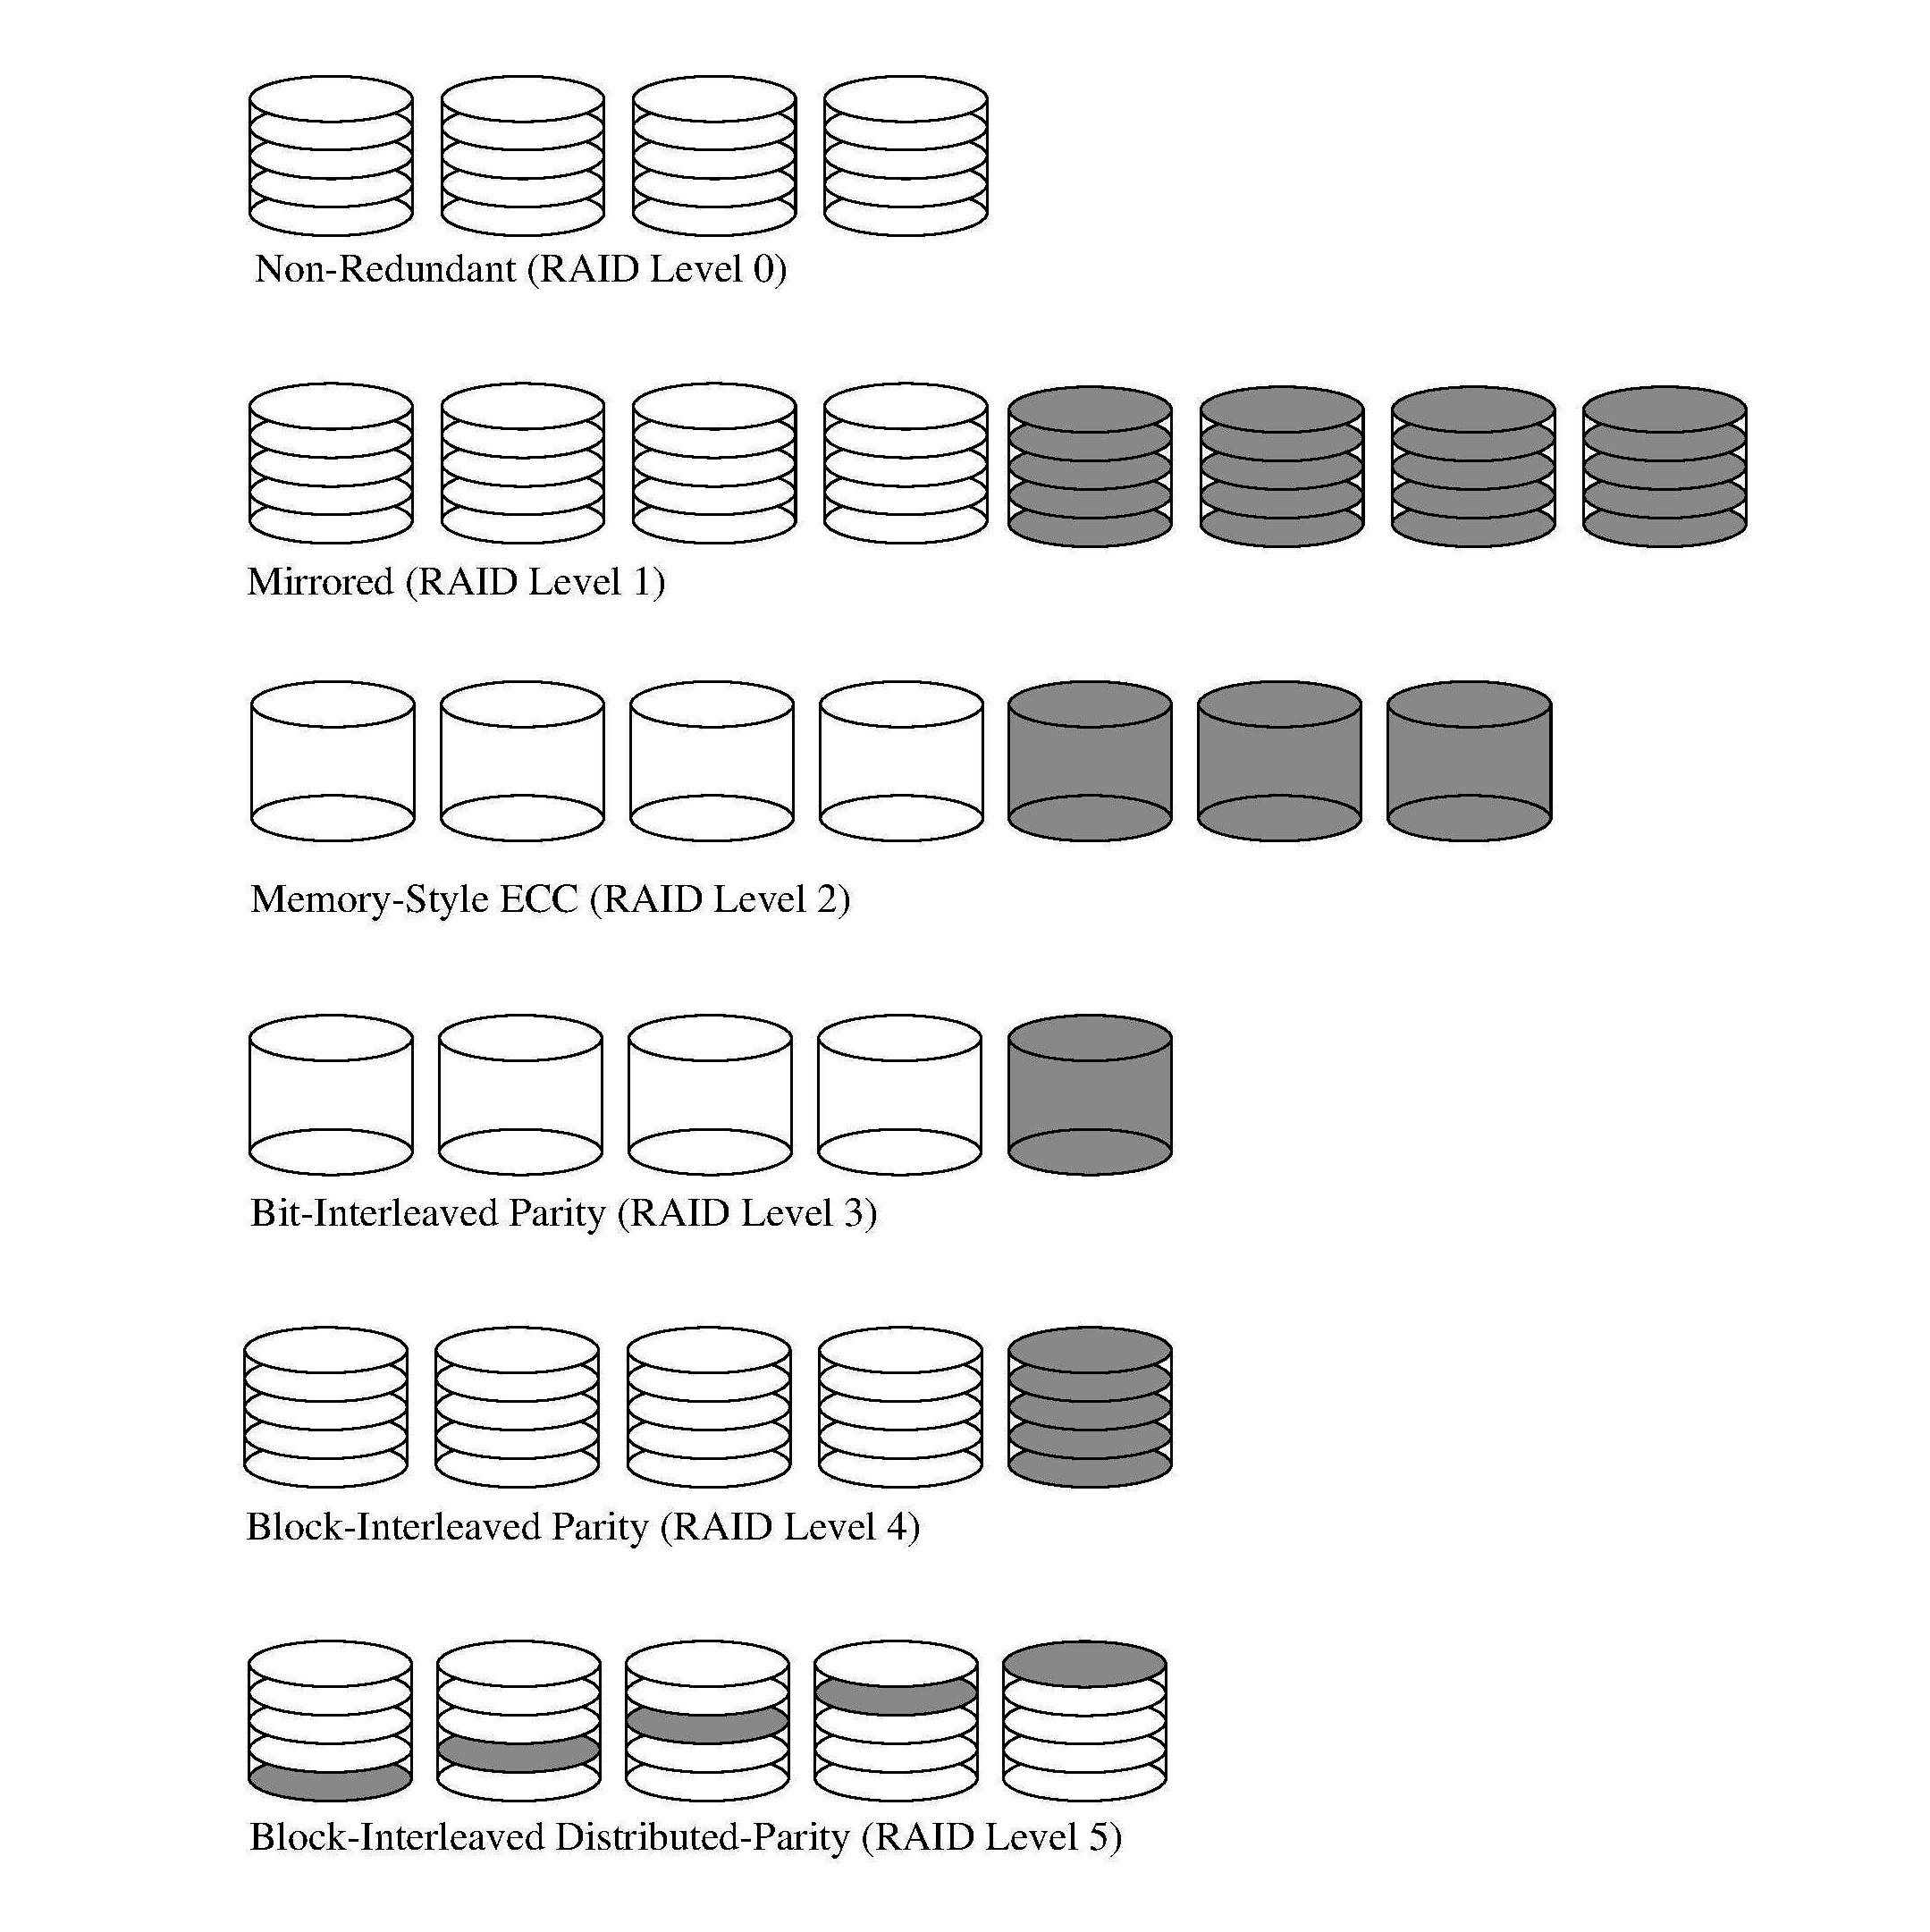
\includegraphics[width=0.6\textwidth]{inleiding-raid-illustratie}
	\caption{Illustratie van verschillende RAID-niveaus \autocite{Chen1994}}
	\label{fig:chen_array_illustratie}
\end{figure}

\subsection{Eigenschappen van RAID-systemen}

Bij het bouwen van RAID-systemen worden er gebruikelijk drie aspecten in beschouwing genomen: \textbf{\gls{performantie}} (performance), \textbf{\gls{betrouwbaarheid}} (reliability) en \textbf{\gls{capaciteit}} (capacity). Een RAID-niveau is in principe niets anders dan een balans tussen deze verschillende eigenschappen; meestal zullen er dus één of meerdere trade-offs moeten gemaakt worden \autocite{Chen1994}.

Begrippen die centraal staan bij RAID zijn \textit{\textbf{striping}} en \textit{\textbf{parity}}. Striping heeft betrekking op de manier waarop een RAID-controller (hetzij hardwarematig, hetzij softwarematig) de blokken data verdeelt over de array van schijven. Bij RAID 0 bijvoorbeeld wordt de data gelijkmatig gedistribueerd volgens het \textit{round-robin}-algoritme \autocite{OSThreePiecesRemzi2015}. Datablokken die verdeeld zijn over meerdere schijven en samen één geheel vormen worden een \textit{stripe} genoemd. \\ 

\subsection{RAID-niveaus: een overzicht}

\subsubsection{RAID 0}

Een voordeel bij RAID 0 is dat de gehele capaciteit van de schijven kan gebruikt worden; er gaat geen ruimte verloren, aangezien de data gelijkmatig verdeeld wordt over de array. Een bijkomend voordeel van striping is dat performantie in het algemeen goed is \autocite{OSThreePiecesRemzi2015} : de meeste en reads en writes kunnen parallel worden afgehandeld. Een voorwaarde voor goede performantie is echter wel dat de \textit{chunk size} (de grootte van de blokken data die worden weggeschreven en/of uitgelezen) ook optimaal wordt gekozen, i.e. afhankelijk van de workload op het systeem \autocite{OSThreePiecesRemzi2015}. Toch kent RAID 0 een groot nadeel: betrouwbaarheid is nagenoeg onbestaande. Aangezien data nergens wordt gedupliceerd, betekent dat het falen van eender welke disk leidt tot verlies van data \autocite{OSThreePiecesRemzi2015}.

\subsubsection{RAID 4}

Parity is een mechanisme dat werd geïntroduceerd bij RAID-niveau 4 om betrouwbaarheid af te dwingen. Bij RAID 4 wordt er metadata over de opgeslagen data bijgehouden in parity blocks op een aparte schijf. Deze metadata wordt verkregen d.m.v. het uitvoeren van een mathematische functie op de opgeslagen data. Meestal is dit een XOR-functie (exclusieve OF) \autocite{Chen1994}. Aan de hand van deze parity kan bij het verlies van één of meerdere schijven de originele data worden gereconstrueerd door XOR'ing toe te passen op de parity bits en de data bits. Bij een XOR-operatie geven een even aantal enen (1) steeds als resultaat nul (0); omgekeerd geldt ook dat een oneven aantal enen (1) steeds een één (1) als resultaat zullen opleveren. Stel dat één schijf van een array van vier schijven faalt, dan kan nog steeds de originele data worden verkregen. Echter, als er meer dan één schijf verloren gaat, dan is het bij RAID 4 onmogelijk om de originele data te herstellen. Het grote voordeel van RAID 4 is dan weer echter dat er minder wordt ingeboet op capaciteit  dan bij bv. RAID 1 en RAID 5 \autocite{OSThreePiecesRemzi2015}. 

\subsubsection{RAID 1}

Naast RAID 0 en RAID 4 zijn er nog andere RAID-levels, zoals RAID 1 en RAID 5. RAID 1 staat ook bekend als \textit{mirroring}, omdat het kopieën maakt van de datablokken naar één of meerdere disks afhankelijk van het aantal schijven. Op gebied van capaciteit is RAID 1 niet echt gunstig, aangezien maar de helft van de totale schijfruimte bruikbaar is. Stel dat er vier schijven in een array aanwezig zijn, dan is slechts de opslagcapaciteit van twee schijven bruikbaar. Daarentegen is de betrouwbaarheid van RAID 1 wel vele malen beter dan die van RAID 0: in theorie mogen er bij een reeks van \textit{n} schijven $\frac{n}{2}$ schijven falen. Maar dan mogen de schijven die elkaars mirror zijn niet falen, want dan is de data op deze disks verloren.  Daarom houdt men in de praktijk meestal de maatstaf van één schijf aan \autocite{OSThreePiecesRemzi2015}.

\subsubsection{RAID 5}

Als laatste wordt RAID 5 besproken. RAID 5 is in principe niets anders dan RAID-niveau 4, maar dan uitgebreid met functionaliteit dat de parity blocks roteert over de verschillende schijven. Dit is een groot verschil t.o.v. RAID 4, waarbij de parity blocks zich op één disk bevinden. Read-performantie is nagenoeg gelijk aan RAID 4, maar write-performantie is stukken beter. Dit komt omdat bij RAID 5 de schrijfoperaties parallel kunnen worden afgehandeld; bij RAID 4 vormt de parity-schijf een \textit{bottleneck} bij het wegschrijven van data \autocite{Chen1994}. De reden hiervoor is dat bij het updaten van data ook de parity blocks moeten worden geüpdatet; alle operaties worden dus m.a.w. serieel uitgevoerd \autocite{OSThreePiecesRemzi2015}.

Er bestaan nog andere, niet-standaard RAID levels, zoals RAID 6 en RAID 10, maar deze worden hier niet besproken.

\section{Inleiding tot ZFS \& RAID-Z}

\subsection{Geschiedenis}

ZFS is een bestandssysteem dat ontwikkeld is door het toenmalige Sun Microsystems, nu onderdeel van Oracle Corporation. Voormalig Sun-werknemer Jeff Bonwick was de oorspronkelijke hoofdontwikkelaar van het bestandssysteem. De ontwikkeling van ZFS startte aan het begin van de jaren 2000; Sun had reeds met de ontwikkeling van bestandssystemen geëxperimenteerd, maar deze pogingen mislukten telkens \autocite{Bonwick2015}. ZFS is een \textit{copy-on-write} (COW) bestandssysteem \autocite{BrianHickmann2007}: bij elke aanpassing van een datablok, wordt het datablok in kwestie niet aangepast, maar wordt het gekopieerd naar een nieuwe locatie en aangepast \autocite{Lucas2015}.

In die tijd gebruikte het bedrijf haar UNIX-besturingssysteem Solaris intern voor verschillende soorten toepassingen, waaronder file servers \autocite{Bonwick2015}. De schijven van deze servers waren opgedeeld in volumes, beheerd door de Solaris Volume Manager (SVM) en geformatteerd in UFS (UNIX Filesystem) \autocite{Bonwick2015}. Toen een verkeerd ingevoerd SVM-commando erin slaagde om het systeem te doen crashen en voor een enorme \textit{downtime} zorgde bij  Sun, was dit voor Bonwick een aanleiding om volledig \textit{from scratch} een bestandssysteem op te bouwen dat makkelijk in gebruik én beheer was.

De hoofdreden om een volledig nieuw bestandssysteem te ontwikkelen was volgens \textcite{JeffBonwick_lastZFS} dat de toenmalige oplossingen voor bestandssystemen totaal achterhaald waren. Bestandssystemen waren nog ontwikkeld voor opslagnoden uit de jaren '80 en '90, welke niet te vergelijken zijn met de huidige noden van zowel bedrijven als particulieren. Naarmate de nood aan meer opslagruimte steeg, moesten er oplossingen worden bedacht, en dit m.b.v. bestandssystemen die hier helemaal niet op voorzien waren. Een 'tussenoplossing', aldus volgens \textcite{JeffBonwick_lastZFS}, die ook vandaag de dag nog gebruikt wordt, is de combinatie van volumes en bestandssystemen. Volumes zijn abstracties voor (delen van) fysieke schijven.

%Een andere eigenaardigheid van bestandssystemen is dat deze nog steeds onlosmakelijk zijn verbonden aan een (deel van) een schijf of opslagapparaat. Volume managers zorgen wel voor een zeker niveau van abstractie, maar bestandssystemen blijven nog steeds gekoppeld aan een bepaalde reeks blokken \autocite{ZFSBonwick}. Dit vonden de ontwikkelaars van ZFS nogal omslachtig: zij zijn van mening dat een bestandssysteem een virtuele abstractie van opslagruimte vormt en dus los moet staan van de fysieke blokken op de schijf. \textcite{ZFSBonwick} maakt de vergelijking met het adresseren van RAM geheugen: RAM-geheugen moet ook eerst niet worden geformatteerd en dan apart worden toegewezen aan applicaties. Bij het alloceren en aanspreken van RAM-geheugen is het immers niet nodig voor de applicatie of programmeur om het exacte geheugenadres te kennen; deze taken worden al afgehandeld door memory allocators m.b.v. virtueel geheugen \autocite{ZFSBonwick}.

%Daarom stelden de ZFS-ontwikkelaars \textit{pooled storage} voor, samen met een geïntegreerde volume manager en storage allocator. Een bijkomend voordeel van \textit{pooled storage} is dat bestandssystemen dynamisch kunnen groeien en verkleinen, zonder tussenkomst van de gebruiker, aangezien de opslagruimte van alle disks als één geheel wordt gezien i.p.v. afzonderlijke eenheden. ZFS maakt het wel mogelijk om quota's in te stellen op bestandssystemen, opdat één bestandssystemen niet alle beschikbare ruimte zou innemen \autocite{ZFSBonwick}. 

\subsection{RAID-Z}

Het ZFS-bestandssysteem omvat ook een softwarematige RAID, RAID-Z genaamd. Volgens \textcite{Bonwick2005} lost RAID-Z in combinatie met ZFS een aantal problemen op die inherent aanwezig zijn bij andere RAID-implementaties. Zo claimen de ontwikkelaars dat RAID-Z het zogenaamde RAID5 \textit{write hole} probleem volledig oplost. Bij klassieke RAID-oplossingen worden stripes weggeschreven op een niet-atomaire manier, i.e. de bewerkingen worden niet als één geheel uitgevoerd. Een bijkomend probleem hierbij is dat bij RAID-levels met \textit{parity} (zoals RAID5) ook nog eens de parity-blocks moeten herberekend worden. Indien het systeem tussen deze bewerkingen crasht of uitvalt door bv. elektriciteitsproblemen, dan bevindt de data op de array van schijven zich in een inconsistente toestand: stripes en parity blocks kunnen corrupt raken \autocite{Bonwick2005}. 

%Een oplossing voor dit probleem is het gebruik van NVRAM waarin stripes tijdelijk kunnen worden bijgehouden. Indien er zich dan een systeemcrash voordoet, dan kan de RAID-controller m.b.v. de gegevens in het NVRAM de originele data herstellen. Maar waar RAID geen oplossing voor heeft, aldus volgens \textcite{Bonwick2005}, is het optreden van \textit{silent data corruption}; de RAID-controller weet immers niet of het al dan niet om corrupte data gaat. Het enige waar een RAID-controller zicht op heeft, zijn blokken. Hiervoor biedt ZFS samen met RAID-Z een oplossing: aangezien het bestandssysteem en RAID-Z samen één geheel vormen, is het mogelijk om van datacorruptie te herstellen of om dit zelfs tegen te gaan. Bij het herstellen van data op de array, overloopt RAID-Z de metadata van het bestandssysteem om zo de stripe-grootte te achterhalen. Ook vergelijkt ZFS bij elk datablok de berekende checksum: indien deze checksums niet overeenkomen, dan tracht ZFS dit blok te repareren m.b.v. de parity-informatie van RAID-Z. Op deze manier kan datacorruptie vroegtijdig worden opgemerkt en kan defecte hardware eventueel vervangen worden \autocite{Bonwick2005}.

\subsection{Toekomst van ZFS}

Ondertussen werd Sun Microsystems overgenomen door Oracle in 2010, na het faillissement van deze eerstegenoemde \autocite{OracleOnbekend}. In 2010 richtten enkele ex-ontwikkelaars van Solaris het illumos-project op met de bedoeling om een volledig open source variant van OpenSolaris te ontwikkelen; ook ZFS werd verder ontwikkeld als onderdeel van illumos \autocite{illumos2012}. De reden hiervoor was dat Oracle geen nieuwe uitgaven meer uitbracht voor OpenSolaris. In 2013 werd het OpenZFS-project opgericht, dat zichzelf als de \textit{"ware en open opvolger van het oorspronkelijke ZFS-project"} ziet \autocite{OpenZFSHistory2014}.

Mede dankzij dit project is ZFS ondertussen beschikbaar op verschillende platformen, waaronder FreeBSD, Linux en macOS.



%%=============================================================================
%% H3 - Ontwerpprincipes van ZFS
%%=============================================================================

\chapter{Ontwerpprincipes \& architectuur van ZFS}
\label{ch:h3}

In dit hoofdstuk worden enkele principes besproken waarop de ontwikkelaars zich hebben gebaseerd bij het ontwerp en de onwtikkeling van ZFS. Tevens wordt de architectuur van ZFS reeds globaal beschreven, om zo de ontwerpbeslissingen van de ontwikkelaars wat meer toe te lichten.

\section{Ontwerpprincipes}

De principes die aan de basis van ZFS liggen vloeiden meestal voort uit de problemen die de ontwikkelaars zelf ervaarden bij het gebruik van andere bestandssystemen.

\subsection{Eenvoud van beheer \& Storage Pools}

Volgens \textcite{ZFSBonwick} kan en moet het aanmaken en beheren van bestandssystemen een stuk makkelijker gemaakt worden. Hierbij speelt automatisatie van verschillende taken een belangrijke rol. Het doel van de gebruiker, nl. \textit{"Het aanmaken van een bestandssysteem"} zou moeten worden vooropgesteld; tevens moet dit proces zo snel een eenvoudig mogelijk verlopen. Ook moet het mogelijk zijn om beheerderstaken (zoals bestandssystemen aanmaken en verwijderen) uit te voeren zonder de werking van het gehele systeem te ondermijnen \autocite{ZFSBonwick}. 

Een niet onbelangrijke feature hierbij zijn storage pools. Storage pools hebben als doel om opslagruimte zoveel mogelijk los te koppelen van de fysieke schijven: alle schijven bevinden zich in een pool van disks. Uit deze pool kunnen bestandssystemen worden aangemaakt, zonder rekening te moeten houden met de limitaties van bv. partities. Tevens kunnen bestandssystemen op een flexibele manier gebruik maken van deze pooled storage door automatisch in te krimpen en uit te breiden wanneer nodig \autocite{ZFSBonwick}. 

\begin{figure}
        \centering
        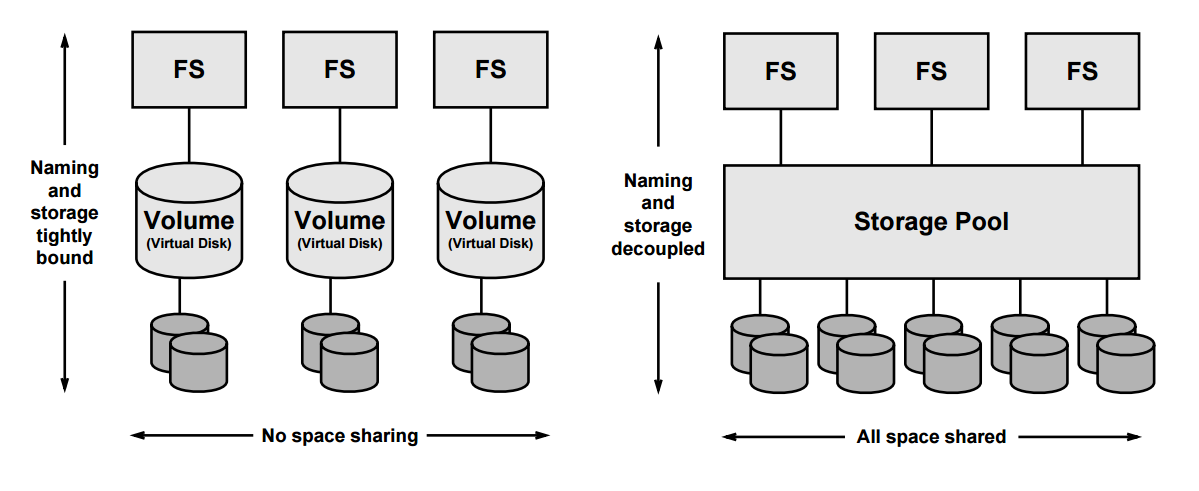
\includegraphics[width=0.8\textwidth]{h3-pools-vs-vols}
        \caption{Illustratie van ZFS pooled storage (rechts) t.o.v.volume-based storage (links) \autocite{ZFSBonwick}}
        \label{fig:bonwick_pools_illustratie}
\end{figure}

\subsection{Consistentie \& Integriteit}

Eén van de taken van een bestandssysteem is om ervoor te zorgen dat het in een consistente toestand blijft, i.e. het moet mogelijk zijn om van inconsistente toestanden te herstellen d.m.v. bijvoorbeeld een journal \autocite{OSThreePiecesRemzi2015}


%%=============================================================================
%% H4 - Het opslagmodel van ZFS
%%=============================================================================

\chapter{Het opslagmodel van ZFS}
\label{ch:h4}

In dit hoofdstuk worden de interne bestandssysteemoperaties van ZFS wat meer toegelicht. Hierbij wordt vooral de werking van de Storage Pool Allocator en de Data Management Unit dieper uitgespit, aangezien deze componenten het beheer van data voor zich nemen.

\section{Structuur van het bestandssysteem}

Datablokken worden bij ZFS voorgesteld als een boomstructuur. Vele andere bestandssystemen, zoals BTRFS op Linux, gebruiken ook boomstructuren voor het bijhouden van data \autocite{Project2017a}. De algemene werking van ZFS en andere, boomgebaseerde bestandssystemen verschillen niet zo heel veel. Echter zijn er ook eigenschappen die uniek zijn aan de manier waarop ZFS de data opslaat.

De belangrijkste elementen van een boom in de informatica zijn de volgende: de wortel (Eng.: \textit{root}), de knopen (Eng.: \textit{nodes}) en de bladeren (Eng.: \textit{leaves}) \autocite{Cohen}. Indien men bij de wortel van een ZFS-boom start, dan komt men als eerste de \textit{\"{u}berblock} tegen: dit is simpelweg een andere benaming voor de wortel van de boom. Dit datablok bevat een checksum van zichzelf en verwijst naar de andere datablokken in de boom. Zoals reeds gezegd in Hoofdstuk \ref{ch:h3}, worden alle blokken gechecksummed om corruptie van data tegen te gaan. Deze checksums worden bewaard in het datablok zelf en in de ouder van de ouder van dit blok: op deze is de hele ketting van datablokken gechecksummed en kan er makkelijk schade worden vastgesteld en kan deze schade eventueel worden gerepareerd. De \textit{\"{u}berblock} is het enige datablok die geen ouder heeft, en dus bewaart deze zijn checksum bij zichzelf \autocite{ZFSBonwick}.  

\section{Checksumming \& Redundantie op blokniveau}




%%=============================================================================
%% H5 - Installatie & Voorbereiding van een Linux-server voor ZFS
%%=============================================================================

\chapter{Opzetten van een testserver voor ZFS}
\label{ch:h5}

In dit hoofdstuk wordt de procedure besproken die werd ondernomen bij het omvormen van een desktopcomputer tot een volwaardige Linux-server die kan gebruikt worden voor ZFS. Nadien worden de stappen besproken voor de installatie van ZFS op deze server.

\section{Gebruikte hardware}

Voor deze scriptie wordt er een HP Pavilion Elite HPE-310be desktopcomputer gebruikt voor te experimenteren met ZFS en het uitvoeren van de testen. Bij het kiezen van een systeem werd er zoveel mogelijk rekening gehouden met de aanbevelingen van de OpenZFS-ontwikkelaars waar mogelijk\footnote{Het gebruikte geheugen beschikt niet over ECC-errorcorrectie; ECC-functionaliteit wordt door de OpenZFS-ontwikkelaars aangeraden om datacorruptie te voorkomen \autocite{OpenZFSProject2017}.}. Wat verder volgt er een overzicht van de specificaties van het gekozen systeem.

\begin{table}
  \centering
  \begin{tabular}{c l}
    \hline
    \multicolumn{2}{c}{\textbf{Specificaties}} \\
    \hline
    Fabrikant & HP \\
    \hline
    Model & HP Pavilion Elite HPE-310be \\
    \hline
    CPU & Intel Core i5 650 @ 3.2 GHz (4 Cores) \\
    \hline
    Geheugen & 10GB DDR3 @ 1333MHz \\
    \hline
    GPU & AMD Radeon HD 5570 \\
    \hline
    \multirow{4}{*}{Interne schijven} & SAMSUNG HD103SJ (1TB) \\
      & WDC WD1002FAEX-0 (1TB) \\
      & WDC WD5000AZRX-0 (500GB) \\
    \hline
    Externe schijf & WD Elements 1078 (1TB) \\
    \hline
    RAID Controller & Intel Corporation SATA RAID Controller \\
    \hline
  \end{tabular}
  \caption{Specificaties van het systeem dat gebruikt wordt doorheen deze bachelorproef (data verkregen via \texttt{lshw})}
  \label{tab:specs_desktop }
\end{table}

\section{Installatie van Linux}

De Linux-distributie die wordt gebruikt doorheen deze scriptie is Fedora 25 Server Edition. De belangrijkste redenen om voor Fedora te kiezen, zijn de volgende:

\begin{itemize}
  \item{Het beschikt over een relatief recente Linux kernel en recente packages;}
  \item{Het is relatief eenvoudig om OpenZFS te installeren op Fedora;}
  \item{De distributie is eenvoudig te installeren}
\end{itemize}

Fedora werd geïnstalleerd op een externe harde schijf via USB: dit om de interne schijven zoveel mogelijk vrij te houden voor ZFS en het uitvoeren van testen. Op de volgende pagina bevindt zich een overzicht van de schijfindeling die gehanteerd werd.

\begin{sidewaysfigure} 
  \Tree
  [.Opslag
      [
        .{Externe\\Opslag}
          [
            .{WD Elements 1078\\(1TB)\\\texttt{(/dev/sdd)}}
                {\texttt{/boot}\\(1GB)\\\texttt{(/dev/sdd1)}}
                [
                  .{\texttt{/dev/sdd2}\\(930.5GB)\\(LVM)}
                    {fedora-swap\\(4.9GB)}
                    {fedora-root\\(15GB)\\\texttt{(/)}}
                    {VRIJE\\RUIMTE\\(910.6GB)}
                ]
          ]
      ]
      [
        .{Interne\\ Opslag}
            {SAMSUNG\\HD103SJ\\(1TB)\\\texttt{/dev/sda}}
            {WDC\\WD1002FAEX-0\\(1TB)\\\texttt{/dev/sdb}}
            {WDC\\WD5000AZRX-0\\(500GB)\\\texttt{/dev/sdc}} 
      ]  !{\qframesubtree} 
  ]
  \caption{Illustratie van de gehanteerde disk-layout van het systeem. De ingekaderde schijven zullen gebruikt worden door ZFS.}
\end{sidewaysfigure}




%%=============================================================================
%% H6 - ZPools & VDEV's
%%=============================================================================

\chapter{Zpools \& VDEV's}
\label{ch:h6}

In dit hoofdstuk worden zpools en diens bouwstenen, VDEV's, wat meer toegelicht. Er wordt ook een demonstratie gegeven over hoe men zpools en VDEV's aanmaakt en wijzigt.

\section{VDEV's: Virtual Devices}

\subsection{Concept}

VDEV's (of voluit Virtual Devices) zijn de bouwstenen van storage pools; het zijn een soort van device drivers die elk een bepaalde functionaliteit aanbieden. Er bestaan verschillende soorten VDEV's: zo zijn er bijvoorbeeld striping VDEV's en mirror VDEV's. Ook worden de verschillende RAID-Z-vormen geïmplementeerd met behulp van één of meerdere VDEV's \autocite{ZFSBonwick}.

Conceptueel worden virtual devices voorgesteld in een boomstructuur, waarvan de bladeren de fysieke VDEV's voorstellen; deze VDEV's komen overeen met fysieke apparaten zoals harde schijven. De andere knopen in de boom worden logische VDEV's genoemd omdat ze een groepering vormen van fysieke VDEV's. Zoals in elke boom bestaat er ook in deze structuur van virtual devices een wortel of \textit{root}. De kinderen van deze root VDEV worden de top-level VDEV's genoemd \autocite{Microsystems2006}.

\begin{figure}
  \centering
  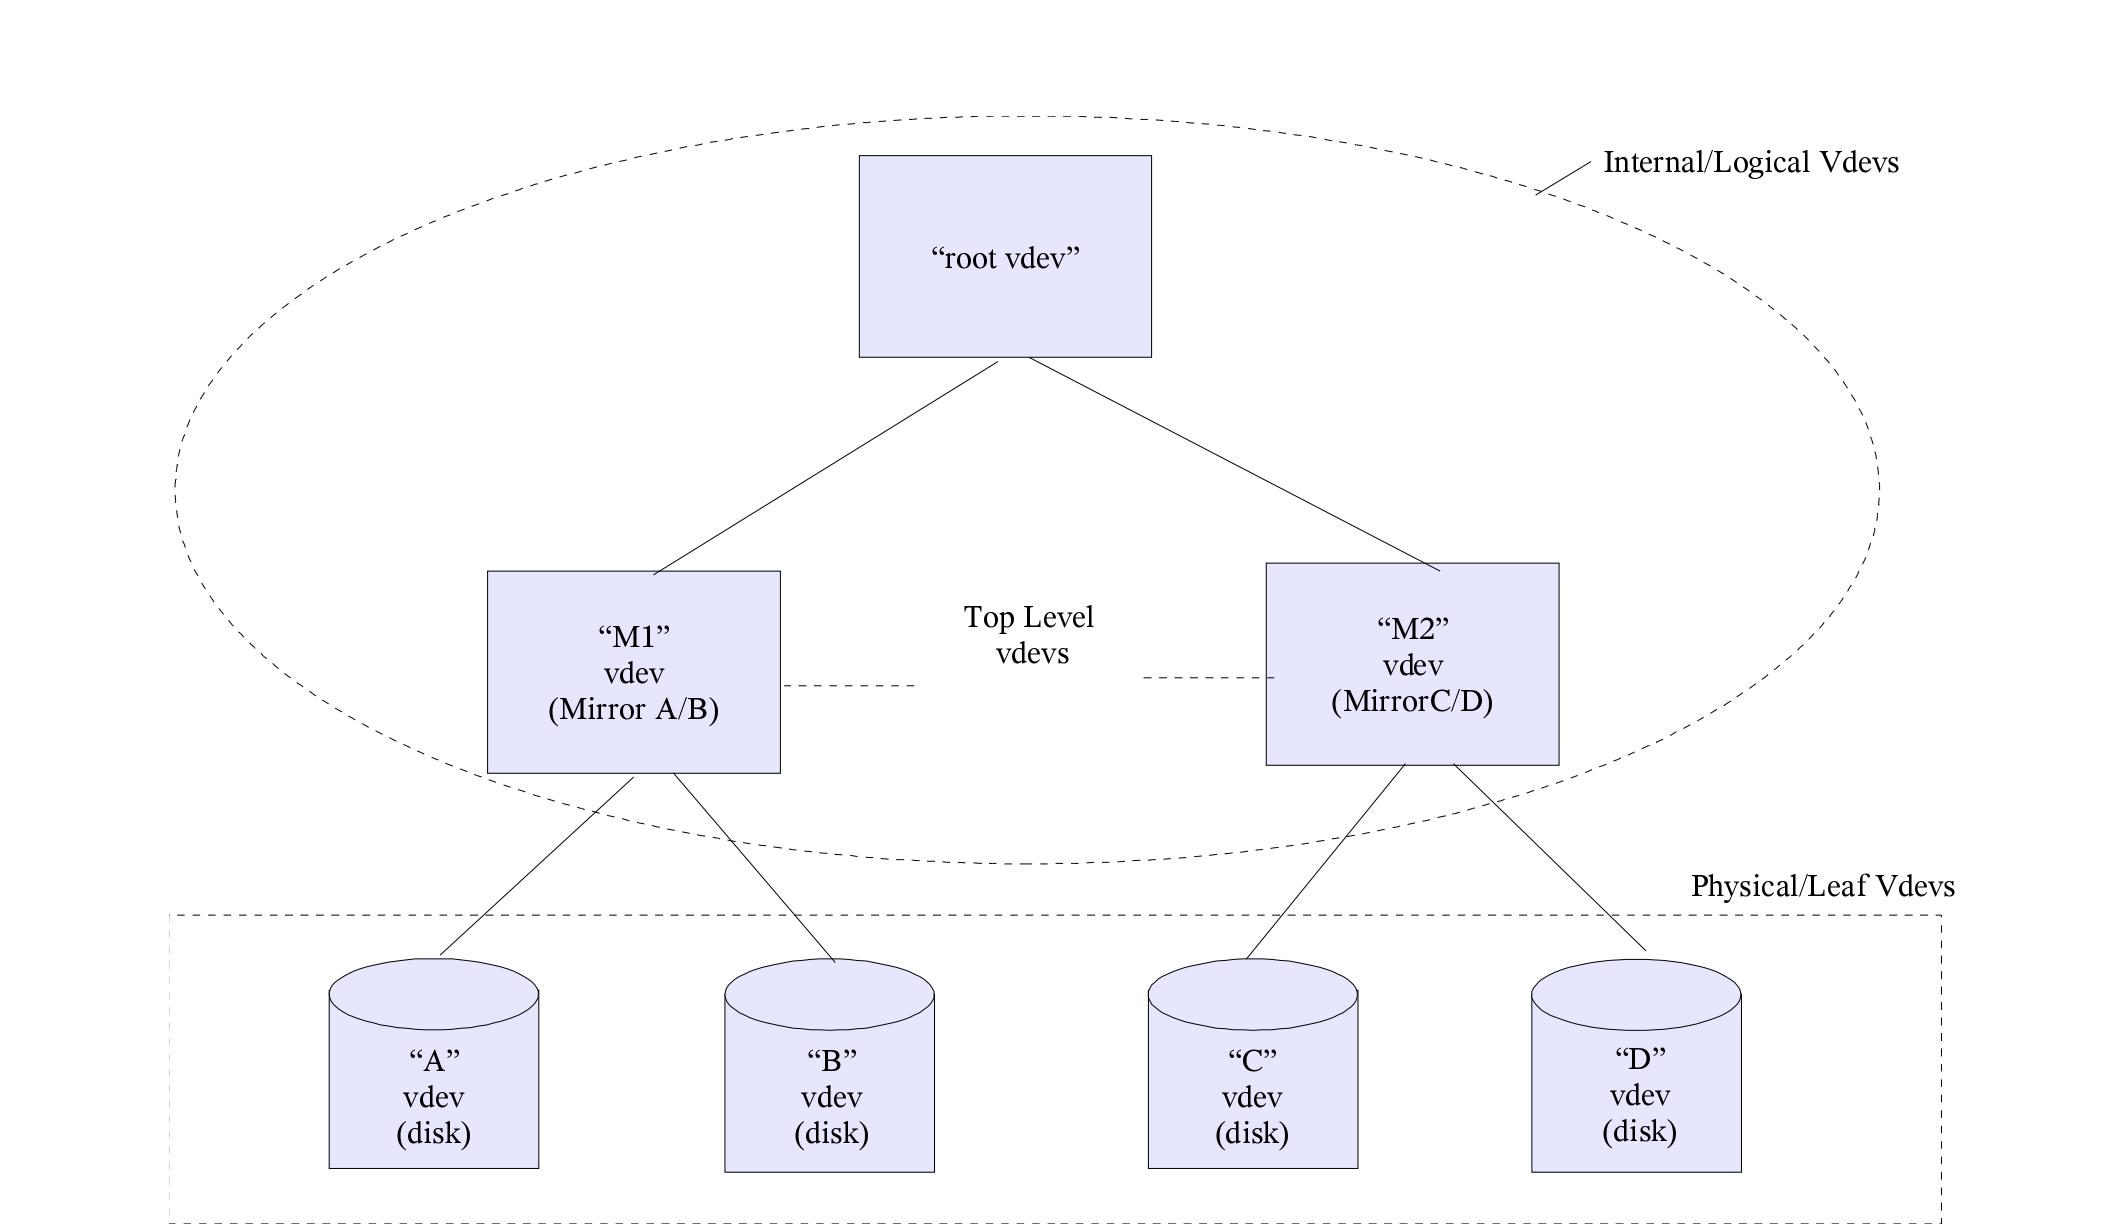
\includegraphics[width=0.9\textwidth]{h6_vdevs_tree}
  \caption{Conceptuele voorstelling van VDEV's in een boomstructuur: M1 en M2 zijn mirrors VDEV's; apparaten A t.e.m. D zijn kinderen van deze VDEV's \autocite{Microsystems2006}.}
  \label{fig:vdevs_boom}
\end{figure}

\subsection{Speciale VDEV's}

Naast VDEV's voor redundantie en striping bestaan er ook nog andere virtual devices die een specifieke rol vervullen. Deze VDEV's worden ingezet met als hoofddoel de performantie van ZFS naar omhoog te trekken \autocite{Lucas2015}.

\subsubsection{SLOG: Seperate Intent Log}

Onder normale omstandigheden bevindt de ZFS Intent Log (ZIL) zich in een pool en worden de bewerkingen die op dit moment bezig zijn naar deze log geschreven. Echter kan de systeembeheerder deze log naar een apart, snel apparaat (zoals een SSD) buiten een pool verplaatsen om zo de performantie omhoog te trekken. ZFS kan logdata effciënter groeperen in batches in plaats van deze weg te schrijven in de volgorde dat de opslagbewerkingen gebeuren; daarna worden deze weggeschreven naar de pool. Dit verhoogt de gehele efficiëntie en snelheid van bewerkingen aanzienlijk. Vele databanksystemen wachten bijvoorbeeld totdat data gepersisteerd is naar de schijf alvorens verder te gaan met een volgende operatie. ZFS kan deze soort operaties loggen en achteraf uitvoeren; het bestandssysteem meldt terwijl aan de databank dat deze operatie gepersisteerd is \autocite{Lucas2015}.

\subsubsection{L2ARC: Level 2 Adaptive Replacement Cache}

Traditioneel gebruiken schijven en bestandssystemen buffers of caches om veelgebruikte data tijdelijk bij te houden; bestandssystemen gebruiken het RAM geheugen om blokken data tijdelijk bij te houden \autocite{OSThreePiecesRemzi2015}. ZFS is hierop geen uitzondering en cachet ook data in het werkgeheugen. Naast dze vorm van caching beschikt ZFS ook over de Adaptive Replacement Cache (ARC). Dit geeft de mogelijkheid om een snel apparaat (zoals een SSD) te gebruiken als extra cache om veelgebruikte bestanden in op te slaan. Het grote verschil met deze manier van bufferen en het gebruik van caches in het RAM-geheugen, is dat in de L2ARC (Level 2 ARC) enkel bestanden worden bijgehouden die frequent gebruikt worden, maar dan weer niet frequent genoeg om in het werkgeheugen te worden bijgehouden \autocite{Lucas2015}. 

\section{Storage pools of zpools}

Zoals reeds gezegd in Hoofdstuk \ref{ch:h3} vormen storage pools (of zpools in ZFS-termen) de eerste vorm van abstractie binnen de gehele ZFS-stack: zpools bieden namelijk een interface aan tot de onderliggende fysieke schijven. Het zijn echter VDEV's die ervoor zorgen dat data kan weggeschreven worden van en naar de schijven. Ter verduidelijking kan er een analogie worden gemaakt met een traditionele RAID-controller en de schijven in een RAID-array: zpools vervullen de rol van RAID-controller, terwijl VDEV's de schijven van de 'array' voorstellen. De zpool ('RAID-controller') verdeelt of stripet data over één of meerdere VDEV's ('schijven') \autocite{Lucas2015}.

\subsection{Aanmaken en beheren van zpools}

Het testsysteem waarover we beschikken bevat drie interne harde schijven, elk direct aangesloten op het moederbord met een SATA-kabel. Dit aantal is voldoende om een RAID-Z1 opstelling mee te maken. Vooraleer er echter VDEV's kunnen worden toegevoegd of gewijzigd, moet er eerst een ZFS storage pool worden aangemaakt; er kunnen meerdere storage pools worden aangemaakt, maar in ons geval is één storage pool meer dan voldoende.

\subsubsection{Bekijken van aanwezige pools}

Voor het beheer van pools wordt er gebruik gemaakt van het commando \texttt{zpool}. Om bijvoorbeeld de huidige zpools te bekijken, geeft men het volgende commando in:

\begin{lstlisting}[language=bash,style=command_style]
$ zpool list
no pools available
\end{lstlisting}

\subsubsection{Aanmaken van een nieuwe pool}

Op dit moment zijn er nog geen pools aangemaakt, dus de uitvoer van bovenstaand commando is normaal. Om een zpool aan te maken met de drie schijven waarover we beschikken, gebruik je het volgende commando:

\begin{lstlisting}[language=bash,style=command_style]
$ zpool create storage /dev/sda /dev/sdb /dev/sdc
\end{lstlisting}

\clearpage

Deze instructie maakt een zpool aan met de naam 'storage'. Vervolgens kan je een lijst opvragen van alle pools die op het systeem aanwezig zijn:

\begin{lstlisting}[language=bash,style=command_style]
$ zpool list
NAME      SIZE  ALLOC   FREE  EXPANDSZ   FRAG    CAP  DEDUP  HEALTH 
storage  2.27T   154K  2.27T         -     0%     0%  1.00x  ONLINE 

(deel van de uitvoer is weggelaten)

\end{lstlisting}

De uitvoer van dit commando geeft reeds enkele eigenschappen van de pool weer, zoals de naam, de totale grootte van de pool, de gebruikte ruimte van de pool, de vrije ruimte en de hoeveelheid fragmentatie. Een andere eigenschap die interessant kan zijn, is DEDUP of deduplicatie: indien er verschillende kopieën zijn van een stuk data, dan houdt ZFS deze maar één keer bij. 

\subsubsection{Gezondheid van pools}

Om de gezondheid en structuur van een pool na te kijken, gebruik je het commando \texttt{zpool status}:

\begin{lstlisting}[language=bash,style=command_style]
$ zpool status
  pool: storage
 state: ONLINE
  scan: none requested
config:

	NAME        STATE     READ WRITE CKSUM
	storage     ONLINE       0     0     0
	  sda       ONLINE       0     0     0
	  sdb       ONLINE       0     0     0
	  sdc       ONLINE       0     0     0

errors: No known data errors
\end{lstlisting}

Dit commando geeft een overzicht van de interne structuur en gezondheid van elke pool op het systeem, samen met de aanwezige VDEV's. Het merendeel van de uitvoer spreekt voor zich: 'pool' geeft de naam van de pool weer en 'state' geeft de algemene toestand van een pool weer. De eigenschap 'scan' geeft aan of er een zogenaamde scrub wordt uitgevoerd of uitgevoerd is geweest. Een scrub is een scan die kan worden uitgevoerd door ZFS om de consistentie en integriteit van de pool na te gaan; indien mogelijk worden fouten automatisch gerepareerd. Een scrub is dus in principe de equivalent voor een \texttt{fsck} binnen ZFS. De vijf kolommen onder de eigenschap 'config' geven informatie over de VDEV's van de pool weer; de drie kolommen aan de rechterzijde geven het aantal fouten aan dat door een bepaald VDEV werd gedetecteerd.

\subsubsection{Eigenschappen van pools}

Zoals reeds gezegd in Hoofdstuk \ref{ch:h3} is ZFS grotendeels een objectgeoriënteerd bestandssysteem. Elk object binnen ZFS heeft bepaalde eigenschappen (properties); deze kunnen dan ook worden opgehaald en gewijzigd. Het is dan ook niet verwonderlijk dat zpools tevens objecten zijn, met elk bepaalde eigenschappen.

Om bijvoorbeeld alle eigenschappen van een pool op te halen, gebruikt men het commando \texttt{zpool get all <naam van de pool>}:

\begin{lstlisting}[language=bash,style=command_style]
$ zpool get all storage
NAME     PROPERTY         VALUE                   SOURCE
storage  size             2.27T                   -
storage  capacity         0%                      -
storage  altroot          -                       default
storage  health           ONLINE                  -
storage  guid             2498162094782357460     default
storage  version          -                       default
storage  bootfs           -                       default
storage  delegation       on                      default
storage  autoreplace      off                     default
storage  cachefile        -                       default
storage  failmode         wait                    default
storage  listsnapshots    off                     default

(deel van de uitvoer is weggelaten)
\end{lstlisting}

Indien men een eigenschap van een pool wilt wijzigen, gebruikt men het commando \texttt{zpool set <eigenschap>=<waarde> <naam van de pool>}: 

\begin{lstlisting}[language=bash,style=command_style]
$ zpool set comment="Testpool" storage
$ zpool get comment storage
NAME     PROPERTY  VALUE     SOURCE
storage  comment   Testpool  local
\end{lstlisting}

In bovenstaand voorbeeld werd de property 'comment' aangepast; vervolgens werd de nieuwe waarde opgehaald.

\subsubsection{Verwijderen van een pool}

Om een zpool en diens VDEV's te verwijderen, gebruik je het commando \texttt{zpool destroy <naam van de pool>}:

\begin{lstlisting}[language=bash,style=command_style]
$ zpool destroy storage
$ zpool list
no pools available
\end{lstlisting}

\clearpage

\subsection{Aanmaken en wijzigen van VDEV's}

In het begin van dit hoofdstuk werd er reeds kort gesproken over VDEV's en hun rol bij zpools: alle redundantie bij RAID-Z zit in feite in deze VDEV's. Het zijn de virtual devices (en dus niet de storage pools) die het maken van een RAID-opstelling binnen ZFS mogelijk maken \autocite{Lucas2015}.

De eigenschappen en principes van de verschillende soorten redundantie VDEV's komen grotendeels overeen met de overeenkomstige standaard RAID-niveaus; deze werden reeds uitvoerig besproken in Hoofdstuk \ref{ch:h2}.

Vooraleer er overgegaan wordt tot het aanmaken van VDEV's, moet er worden opgemerkt dat de structuur van zpools en van de meeste VDEV's na creatie vast ligt. Zpools kunnen uitgebreid worden met meer schijven en/of partities en VDEV's, maar aan een VDEV kan men in de meeste gevallen geen apparaten toevoegen \autocite{FBSDDP2017}. 

\subsubsection{Striping VDEV's}

Striping VDEV's komen overeen met RAID-niveau 0; bij zpools bestaande uit striping VDEV's wordt data gelijkmatig verdeeld over de verschillende VDEV's.

In de voorgaande sectie over zpools werden er bij het aanmaken van een nieuwe zpool impliciet striping VDEV's gebruikt:

\begin{lstlisting}[language=bash,style=command_style]
$ zpool create storage /dev/sda /dev/sdb /dev/sdc
$ zpool status
  pool: storage
  state: ONLINE
  scan: none requested
  config:

	NAME        STATE     READ WRITE CKSUM
	storage     ONLINE       0     0     0
	  sda       ONLINE       0     0     0
	  sdb       ONLINE       0     0     0
	  sdc       ONLINE       0     0     0

  errors: No known data errors
\end{lstlisting}

In dit geval wordt elke fysieke harde schijf in een aparte VDEV gestopt en wordt de data gelijkmatig verdeeld over de drie VDEV's (\texttt{sda}, \texttt{sdb} en \texttt{sdc}).

\subsubsection{Mirror VDEV's}

Bij mirror VDEV's zijn de kinderen van de VDEV's kopieën van elkaar: dit is hetzelfde principe dat bij RAID 1 wordt toegepast. 

Mirrors zijn overigens de enige VDEV's waaraan die men na creatie nog kan wijzigen, samen met stripes. Aan een mirror VDEV kunnen achteraf nog schijven worden toegevoegd; een striping VDEV kan worden geüpgradet tot een mirror VDEV door een extra schijf of schijven aan de VDEV toe te voegen \autocite{FBSDDP2017}.

We beschikken bijvoorbeeld over de volgende storage pool met één striping VDEV, bestaande uit één fysieke schijf:

\begin{lstlisting}[language=bash,style=command_style]
$ zpool create storage /dev/sda
$ zpool status
  pool: storage
  state: ONLINE
  scan: none requested
  config:

	NAME        STATE     READ WRITE CKSUM
	storage     ONLINE       0     0     0
	  sda       ONLINE       0     0     0

  errors: No known data errors
\end{lstlisting}

Deze striping VDEV kan makkelijk worden geüpgradet naar een mirror VDEV m.b.v. het commando \texttt{zpool attach <naam pool> <naam VDEV> <schijf>}:

\begin{lstlisting}[language=bash,style=command_style]
$ zpool attach storage sda sdb
$ zpool status
  pool: storage
  state: ONLINE
  scan: resilvered 59.5K in 0h0m with 0 errors on Tue May  9 17:16:23 2017
  config:

	NAME        STATE     READ WRITE CKSUM
	storage     ONLINE       0     0     0
	  mirror-0  ONLINE       0     0     0
	    sda     ONLINE       0     0     0
	    sdb     ONLINE       0     0     0

  errors: No known data errors
\end{lstlisting}

Bij het weergeven van de structuur van de pool, kan men zien dat de stripe werd geüpgradet naar een mirror, met \texttt{sda} en \texttt{sdb} als kinderen. Ook werd er een scrub uitgevoerd na het toevoegen van de nieuwe schijf.

\subsubsection{RAID-Z1 VDEV's}

Aangezien het testsysteem over slechts drie fysieke schijven beschikt, kunnen we niet verder gaan dan RAID-niveau 5\footnote{In theorie zou er kunnen gebruikt gemaakt worden van binary files als storage-backend; ZFS kan namelijk bestanden gebruiken als provider. Maar aangezien deze bestanden op de externe harde schijf zouden moeten worden opgeslagen, zou dit de performantie te sterk naar beneden halen (de schijf is aangesloten via USB 2.0).}. Het equivalent van RAID 5 bij ZFS is RAID-Z1.  

Om een RAID-Z1 VDEV te kunnen creeëren, dienen eerst de bestaande VDEV's worden verwijderd. Het makkelijkste is om de bestaande pool volledig te verwijderen en een nieuwe pool met een RAID-Z1 VDEV aan te maken:

\begin{lstlisting}[language=bash,style=command_style]
$ zpool destroy storage
$ zpool create storage raidz1 /dev/sda /dev/sdb /dev/sdc
$ zpool status
  pool: storage
  state: ONLINE
  scan: none requested
  config:

	NAME        STATE     READ WRITE CKSUM
	storage     ONLINE       0     0     0
	  raidz1-0  ONLINE       0     0     0
	    sda     ONLINE       0     0     0
	    sdb     ONLINE       0     0     0
	    sdc     ONLINE       0     0     0

  errors: No known data errors
\end{lstlisting}

Er zijn nog andere RAID-Z VDEV's mogelijk, zoals RAID-Z2 (equivalent van RAID 6) en RAID-Z3. Deze vereisen echter vier schijven of meer en zijn dus niet mogelijk in combinatie met het testsysteem.

\subsubsection{SLOG \& L2ARC VDEV's}

Typisch wordt er een klein en snel opslagapparaat - zoals een SSD - gebruikt voor de SLOG en L2ARC. Om te demonstreren hoe de indeling van een pool met één van deze VDEV's er zou uitzien, wordt er telkens een mirror VDEV aangemaakt samen met respectievelijk een SLOG VDEV en een L2ARC VDEV. Een SLOG VDEV kan worden gemirrored; een L2ARC VDEV niet \autocite{FBSDDP2017}.

Eerst en vooral moet de bestaande pool worden verwijderd; nadien kan een nieuwe pool met de nodige VDEV's worden aangemaakt:

\begin{lstlisting}[language=bash,style=command_style]
$ zpool destroy storage
$ zpool create storage mirror /dev/sda /dev/sdb log /dev/sdc
$ zpool status
  pool: storage
 state: ONLINE
  scan: none requested
config:

	NAME        STATE     READ WRITE CKSUM
	storage     ONLINE       0     0     0
	  mirror-0  ONLINE       0     0     0
	    sda     ONLINE       0     0     0
	    sdb     ONLINE       0     0     0
	logs
	  sdc       ONLINE       0     0     0

  errors: No known data errors
\end{lstlisting}

In bovenstaand voorbeeld ziet men mooi dat SLOG VDEVS zich buiten een pool bevinden. Ook is er in dit geval een duidelijk onderscheid tussen logische en fysieke VDEV's: \texttt{mirror-0} en \texttt{logs} zijn logische VDEV's, terwijl \texttt{sda}, \texttt{sdb} en \texttt{sdc} fysieke VDEV's zijn. Men ziet ook dat het mogelijk is om bij de creatie van een pool onmiddellijk alle VDEV-definities mee te geven.

Het aanmaken van een caching VDEV verloopt gelijkaardig:

\begin{lstlisting}[language=bash,style=command_style]
$ zpool destroy storage
$ zpool create storage mirror /dev/sda /dev/sdb cache /dev/sdc
$ zpool status
  pool: storage
 state: ONLINE
  scan: none requested
config:

	NAME        STATE     READ WRITE CKSUM
	storage     ONLINE       0     0     0
	  mirror-0  ONLINE       0     0     0
	    sda     ONLINE       0     0     0
	    sdb     ONLINE       0     0     0
	cache
	  sdc       ONLINE       0     0     0

  errors: No known data errors
\end{lstlisting}

Ook hier bevindt de L2ARC VDEV zich buiten de pool en kan opnieuw de indeling tussen fysieke en logische VDEV's duidelijk worden opgemerkt.


%%=============================================================================
%% Conclusie
%%=============================================================================

\chapter{Conclusie}
\label{ch:conclusie}

%% TODO: Trek een duidelijke conclusie, in de vorm van een antwoord op de
%% onderzoeksvra(a)g(en). Wat was jouw bijdrage aan het onderzoeksdomein en
%% hoe biedt dit meerwaarde aan het vakgebied/doelgroep? Reflecteer kritisch
%% over het resultaat. Had je deze uitkomst verwacht? Zijn er zaken die nog
%% niet duidelijk zijn? Heeft het ondezoek geleid tot nieuwe vragen die
%% uitnodigen tot verder onderzoek?

%\lipsum[76-80]

Doorheen deze bachelorproef is het (hopelijk) duidelijk geworden dat het gebruik van de term 'bestandssysteem' ZFS eigenlijk een beetje onrecht aandoet. De afkorting 'ZFS' mag dan wel Zettabyte Filesystem betekenen, toch is ZFS veel meer dan een bestandssysteem alleen: het is een volledig nieuwe implementatie van de traditionele opslagstack zoals we die al jaren gewend zijn. Daar waar meer traditionele oplossingen vaak bestaan uit verschillende, losse onderdelen die met elkaar samenwerken, bestaat de ZFS storage stack uit een aantal nauw samenwerkende lagen. Toch voelt dit niet aan als een groot, log geheel; functionaliteiten zijn duidelijk afgebakend en dit weerspiegelt zich ook in het gebruik en beheer.   

Toen ZFS voor het eerst op het toneel verscheen, waren vele techneuten laaiend enthousiast: problemen zoals datacorruptie en inflexibele opslag zouden eindelijk van de baan zijn.  


%%---------- Back matter ------------------------------------------------------

\printbibliography
\addcontentsline{toc}{chapter}{\textcolor{maincolor}{\IfLanguageName{dutch}{Bibliografie}{Bibliography}}}

% Woordenlijst
\printnoidxglossaries

\listoffigures
\listoftables

\end{document}
